\documentclass[40pt,letterpaper,physrev]{article}
\usepackage[utf8]{inputenc}
\usepackage{float}
\usepackage{graphicx}
\usepackage{amsmath}
\usepackage{amsfonts}
\usepackage{amssymb}
\usepackage{cancel}
\usepackage{times} % set times font
\usepackage{color}
\usepackage{datetime}
\usepackage{fullpage}
\usepackage{tikz}
\usepackage{caption}
\usepackage{url}
\DeclareGraphicsExtensions{.pdf,.png,.jpg,.eps} 
\author{Dmitri Priimak}
\title{On high-frequency signal amplification in semiconductor super-lattice in cross electric and magnetic fields 
at finite temperatures}
\begin{document}
\bibliographystyle{plain}
\newcommand{\ddx}[2] {
	\frac{\text{d}#1}{\text{d}#2}
}
\newcommand{\ddt}[1] {
	\frac{\text{d}#1}{\text{d}t}
}
\newcommand{\dtwodt}[1] {
	\frac{\text{d}^{2}#1}{\text{d}t^{2}}
}
 \begin{center}
  {\bf On high-frequency signal amplification in semiconductor super-lattice in cross electric and magnetic fields 
at finite temperatures}
 \end{center}
  \begin{abstract}
  We analyze numerically small signal amplification in semiconductor super-lattice at finite temperatures in cross
electric and magnetic fields. We predict significant amplification in cyclotron regime, when electrons do not reach
edges of Brillouin zone due to folding of electron distribution function under influence of magnetic field. Also
predicted week low frequency amplification at higher temperatures in a narrow set of parameters when distribution
function overflows slightly over the edges of Brillouin zone.
  \end{abstract}
  \section{Introduction}  
A semiconductor super-lattice (SL), first studied by Esaki and Tsu \cite{Esaki:70}, is an artificial periodic structure, with periods
much larger than possible in the normal crystals. It offers may opportunities for industrial applications, most of which
have not been realized for variety of reasons. More fruitful were applications of SL to the study of fundamental
properties of solids. Crucial property of SL is narrowness of conduction band, often referred as ”mini-band”, which
allows electrons to transit this zone several times before experiencing collision with the crystal lattice. This property
offered one of the earliest ways to observe, so called ”Bloch oscillations” \cite{BLOCH}, which would allow generation of
high frequency emf fields. This however did not come to fruition as there are mechanisms that destroy these oscillations,
one of which is formation of electron domains [*] as well very small power output of such devices [*].
Another very promising field is in observing reaction of SL to the external a/c emf with very practical possibilities
of signal detection and amplification. Non-linearity of energy dispersion relation in the mini-band, exposed to use due
to the narrowness of the mini-band, offers many intriguing possibilities for study of chaos \cite{Alekseev2002281} and high frequency signal amplification \cite{PhysRevB.77.165330}. Several different experiments were already 
performed \cite{PhysRevB.56.10303}, but almost infinite number of possible
configurations presents a challenge and makes it all the more important farther theoretical and numerical investigation.
Detailed review of SL theory and known analytical solutions can be found in work by A. Wacker \cite{WAC01}.
In out work we look at SL, using semi-classical theory, under action of electric field 
$E(t) = E_{dc} + E_{\omega}\cos(\omega t)$ along the superlattice axis and constant perpendicular magnetic field.
  	\begin{figure}[H]
	  \centering
	  \normalsize % use normal font size in the figure
	  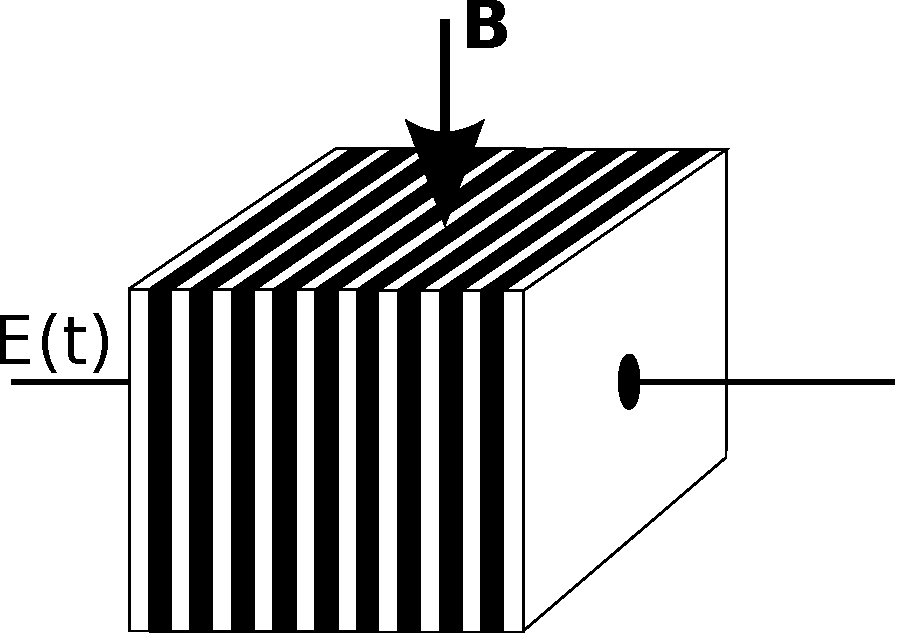
\includegraphics[scale=0.7]{illustrations/SL_CROSS_E_AND_B.pdf}
	  \caption{}
	\end{figure}
    The gist of this configuration is presence of two types of motion of electrons in the SL, cyclotron-like like motion
    and, what we may call, Bloch oscillation regime, also modified due to the presence of magnetic field. This
    configuration has already been studied in the limiting case of zero temperature \cite{PhysRevLett.103.117401}. We,
    however, will be looking at non-zero temperature, all the way up to the room temperature.
  \section{Analytical treatment}
    We take approach of semi-classical theory based on Boltzmann equation, where, the entirety of quantum 
    mechanical nature of the SL is hidden in electron velocity $\mathbf{v}(\mathbf{k})$, which is a function of $
    \mathbf{k}$, crystal momentum. 
    \begin{equation}\label{eq:boltzmann}
     \frac{\partial f}{\partial t}+
     \frac{e}{\hbar}\left ( \mathbf{E} + \mathbf{v}\times\mathbf{B} \right ) \frac{\partial f}{\partial\mathbf{k}}+
     \mathbf{v}(\mathbf{k})\frac{\partial f}{\partial r} = \left ( \frac{\partial f}{\partial t} \right )_{st}
    \end{equation}
    Where $\left ( \partial f/\partial t \right )_{st}$ is a collision term responsible for relaxation to the
    normal electron density distribution function in the absence of external fields. Here we consider the simplest
    form of this term $(f_0-f)/\tau$. Where $f_0$ is, in general, Fermi distribution, but at finite temperatures
    can be approximated by Boltzmann distribution.
    Since we consider electron density $f$ to be spatially homogeneous, $f$ depends only on $\mathbf{k}$ and 
    Boltzmann equation takes form
    \begin{equation}\label{eq:boltzmann_homo}
     \frac{\partial f}{\partial t}+
     \frac{e}{\hbar}\left ( \mathbf{E} + \mathbf{v}\times\mathbf{B} \right ) \frac{\partial f}{\partial\mathbf{k}}
     = \frac{f_0 - f}{\tau}
    \end{equation}
    Electric field is along x-axis and magnetic field is along z-axis.
    \begin{align}
     \mathbf{E}=&(E,0,0) \\
     \mathbf{B}=&(0,0,B) \\
     \mathbf{v}\times\mathbf{B}=&(v_y B, -v_x B, 0))
    \end{align}
    We now proceed with making variety of substitutions to turn this equation into dimensionless form. First we
    will make following substitution
    \begin{equation}
     t \to \tau t
    \end{equation}
    which gives following form to the Boltzmann equation
    \begin{equation}
     \frac{\partial f}{\partial t}+
     \frac{ed\tau}{\hbar}(E+v_{y}B)\frac{\partial f}{\partial(k_x d)}-
     \frac{ed\tau}{\hbar}v_{x}B\frac{\partial f}{\partial(k_y d)}
     = f_0 - f
    \end{equation}
    where 
    \begin{equation}
     \mathbf{v}=\frac{1}{\hbar}\frac{\partial\varepsilon}{\partial\mathbf{k}}
    \end{equation}
    and $\varepsilon$ is an energy of an electron in the zone, which in tight-binding apporiximation takes form in the first zone
    \begin{equation}
     \varepsilon=\frac{\hbar^2k^2_y}{2m}-\frac{\Delta_{1}}{2}\cos(k_{x}d)\label{eq:energy_unscaled}
    \end{equation}
    therefore
    \begin{align}
     v_x=&\frac{\Delta_{1}d}{2\hbar}\sin(dp_x/h) \\
     v_y=&\frac{\hbar k_y}{m}
    \end{align}
    And Boltzmann equations now takes following form
   \begin{equation}
     \frac{\partial f}{\partial t}+
     \left ( \frac{ed\tau}{\hbar}E+\frac{ed\tau}{m}k_yB \right ) \frac{\partial f}{\partial(k_x d)}-
     \frac{\Delta_{1}ed^2\tau}{2\hbar^2}B\sin(k_{x}d)\frac{\partial f}{\partial(k_y d)}
     = f_0 - f
   \end{equation}
   Now we can define
   \begin{align}
	E_*=&\frac{\hbar}{ed\tau} \\	
	m_x=&\frac{2\hbar^2}{\Delta_1 d^2} \\
   \end{align}
   \begin{equation}
	\boxed{\alpha=m/m_x}\label{eq:alpha_def}
   \end{equation}
   Then, with cyclotron frequency defined as 
   \begin{equation}
	\omega_c=\frac{eB}{\sqrt{mm_x}}
   \end{equation}
   we get following
   \begin{equation}
     \frac{\partial f}{\partial t}+
     \left ( \frac{E}{E_*}+\frac{\omega_{c}\tau}{\sqrt{\alpha}}k_yd \right ) \frac{\partial f}{\partial(k_x d)}-
     \sqrt{\alpha}\omega_c\tau\sin(k_x d)\frac{\partial f}{\partial(k_y d)}
     = f_0 - f
   \end{equation}
   And if we now define
   \begin{align}
       \phi_x=&k_{x}d \\
       \phi_y=&\frac{k_{y}d}{\sqrt{\alpha}} \\
       \tilde{E}=&E/E_*\\
       \tilde{B}=&\omega_{c}\tau
   \end{align}
   Boltzmann equations takes form
   \begin{equation}
   	\boxed{
   	\label{eq:boltzmann_final}
     \frac{\partial f}{\partial t}+
     \left ( \tilde{E}+\tilde{B}\phi_y\right ) \frac{\partial f}{\partial\phi_x}-
     \tilde{B}\sin(\phi_x)\frac{\partial f}{\partial\phi_y}
     = f_0 - f}
   \end{equation}
   Alternatively, if we define Bloch frequency as
   \begin{equation}
	\omega_B=\frac{edE}{\hbar}
   \end{equation}
   it can be written as 
   \begin{equation}
     \frac{\partial f}{\partial t}+
     \left ( \omega_B\tau+\omega_c\tau\phi_y\right ) \frac{\partial f}{\partial\phi_x}-
     \omega_c\tau\sin(\phi_x)\frac{\partial f}{\partial\phi_y}
     = f_0 - f
   \end{equation} 
    Ratio of Bloch and cyclotron oscillation frequencies will be important to us down the road.
    For $f_0$ we use Boltzmann distribution 
    \begin{equation}
        f_0\propto e^{\displaystyle -\frac{\varepsilon}{k_bT}}
    \end{equation}
    which in our variables $\phi_x$ and $\phi_y$ takes form
    \begin{equation}
	f_0=C\exp{\left \{ \mu\cos(\phi_x)-\frac{\mu}{2}\phi^2_y\right \} }
	\end{equation}
	\begin{equation}
	\boxed{\mu=\frac{\Delta_1}{2k_{b}T}}
    \end{equation} 
    Now, constant $C$ must be such that dimensionless norm of $f_0$ is 1. Therefore
    \begin{align}
       \frac{1}{C}=&\frac{d^2}
	{\hbar^2}\int^{+\infty}_{-\infty}\text{d}p_y\int_{p_x\in\text{BZ}}\text{d}p_x
	\exp{\left \{ \mu\cos(\phi_x)-\frac{\mu}{2}\phi^2_y\right \} } \\
	   =&\sqrt{\alpha}\int^{+\infty}_{-\infty}e^{-\mu\phi^2_y/2}\text{d}\phi_y
	   \int^{\pi}_{-\pi}e^{\mu\cos(\phi_x)}\text{d}\phi_x \\
	   =&2\pi I_0(\mu)\sqrt{\frac{2\pi\alpha}{\mu}}
    \end{align}
    Thus, full form of equilibrium distribution is
    \begin{equation}
    \boxed{
	f_0=\frac{1}{2\pi I_0(\mu)}\sqrt{\frac{\mu}{2\pi\alpha}}\exp{\left \{ \mu\cos(\phi_x)-\frac{\mu}{2}\phi^2_y\right \} } }
	\end{equation}
	This way, in total, we have four free parameters defining our system, $\mu$ and $\alpha$ that characterize lattice parameters such as lattice period and band width and temperature, and $\tilde{E}$, $\tilde{B}$ that specify external fields.
	One of the parameters that we will be calculating is drift 
	velocity $v_{dr}$, which we will define like this
	\begin{align}
		v_{dr}=&\frac{2d}{\Delta_1\hbar}\iint
			\frac{\partial\varepsilon}{\partial p_x}f(p_x,p_y)\text{d}p_x\text{d}p_y \\
			=&\sqrt{\alpha}\int^{\pi}_{-\pi}\text{d}\phi_x\int^{+\infty}_{-\infty}\text{d}\phi_y\sin(\phi_x)f(\phi_x,\phi_y)\label{eq:v_dr_generic}
	\end{align}
    When magnetic field is $0$ and $E$ is constant, i.e. $E_{dc}$, analytic 
    solution Boltzmann equation is well known and as well as expression for 
    drift velocity and absorption (see below) \cite{WAC01}
    \begin{align}
	v_{dr}=&\left \{ \sqrt{\alpha}\int^{\pi}_{-\pi}\text{d}\phi_x\int^{+\infty}_{-\infty}\text{d}\phi_y\sin(\phi_x)f_0(\phi_x,\phi_y)\right \}
	\frac{E_{dc}/E_*}{1+(E_{dc}/E_*)^2} \\
	=&\frac{I_1(\mu)}{I_0(\mu)}\frac{E_{dc}/E_*}{1+(E_{dc}/E_*)^2}
    \end{align}
	From which follows that peak value of $v_{dr}$ is at $E_{dc}/E_*=1$ and is 
	\begin{equation}
		v_p=\frac{I_1(\mu)}{2I_0(\mu)}\label{eq:v_peak}
	\end{equation}
	Later, down the road, we will be plotting not $v_{dr}$, but $v_{dr}/v_p$,
	which for dc electric field only take very simple form, known as "Esaki-Tsu" equation
	\begin{equation}
		\frac{v_{dr}}{v_p}=2\frac{E_{dc}/E_*}{1+(E_{dc}/E_*)^2}
	\end{equation}
	In general we will be applying a/c emf in the form 
	\begin{equation}
	\tilde{E}=\tilde{E}_{dc}+\tilde{E}_{\omega}\cos(\omega t)\label{eq:tilde_E_as_a_function_of_time}
	\end{equation}
	and in case when magnetic field is not applied we also have analytic expression for $v_{dr}$, which is known as "Tien-Gordon" equation. In the presence of a/c emf we compute absorption $A$ and dispersion $ASIN$, which are defined as 
	\begin{equation}
	A=\left <\frac{v_{dr}}{v_p}\cos(\omega t) \right >_{t}
	\end{equation}
    In the absence of magnetic field, analytic expression for absorption known as "Taker formulae" \cite{WAC01}. 
    Not much analytically known, however, when magnetic field is applied.
    	
	Now due to periodicty of $f(\phi_x,\phi_y)$ along $\phi_x$ with 
	period $2\pi$ and additionally 
	$f_0(-\phi_x, \phi_y)=f_0(\phi_x, \phi_y)$, it makes sense 
	for us to expand $f$ and $f_0$ into Fourier series.
	\begin{align}
		f_0=&\sum^\infty_{n=0}a^{(0)}_{n}\text{cos}(n\phi_x)\label{eq:f0_fourier_representation} \\
		f=&\sum^\infty_{n=0}a_{n}\text{cos}(n\phi_x)+
		b_{n}\text{sin}(n\phi_x)\label{eq:f_fourier_representation}
	\end{align}
	where coeffients $a^{(0)}_n$, $a_n$ and $b_n$ in general will depend on $\phi_y$ and last two also on time $t$. Note, that $a_{n<0}\equiv 0$ and $b_{n<1}\equiv 0$. And with the from of $f_0$, as selected above, $a^{(0)}_n$ becomes
	\begin{align}
		a^{(0)}_n=&\frac{\sigma(n)}{\pi}\int^{\pi}_{-\pi}f_0(\phi_x,\phi_y)\cos(n\phi_x)\text{d}\phi_x \\
		=&\frac{\sigma(n)I_n(\mu)}{\pi I_0(\mu)}\sqrt{\frac{\mu}{2\pi\alpha}}\exp{\left \{ -\frac{\mu}{2}\phi^2_y\right \} }
	\end{align}
	where 
	\begin{equation}
		\sigma(n)=
		\begin{cases}
   		1/2 & : n=0 \\
   		1 & : n\ne 1
  		\end{cases}
	\end{equation}
	Norm of $f(\phi_x,\phi_y)$ must always be one, i.e.
	\begin{equation}
		\sqrt{\alpha}\int^{\pi}_{-\pi}\text{d}\phi_x
			\int^{+\infty}_{-\infty}\text{d}\phi_y f(\phi_x,\phi_y)=1
	\end{equation}
	which in fourier representation takes form
	\begin{equation}
	\boxed{
		2\pi\sqrt{\alpha}\int^{+\infty}_{-\infty}a_0(\phi_y)\text{d}
		\phi_y=1}
	\end{equation}
	Once we move on to the numerical calculations this equation can be used to check correctness. And from equation (\ref{eq:v_dr_generic}) it is clear that only $b_1$ will survice. And calculation of $v_{dr}$ is done through following 
	equation
	\begin{align}
		v_{dr}=&\sqrt{\alpha}\int^{+\infty}_{-\infty}\text{d}\phi_{y}\int^{+\pi}_{-\pi}\text{d}\phi_x\sin(\phi_x)b_1(\phi_y)\sin(\phi_y)\\
		=&\pi\sqrt{\alpha}\int^{+\infty}_{-\infty}b_1(\phi_y)\text{d}\phi_y
	\end{align}
	and in view of definition of peak value of $v_{dr}$ in eq. (\ref{eq:v_peak})
	\begin{equation}
	\boxed{
		\frac{v_{dr}}{v_p}=\frac{2I_0(\mu)\pi\sqrt{\alpha}}{I_1(\mu)}
			\int^{+\infty}_{-\infty}b_1(\phi_y)\text{d}\phi_y
			}
	\end{equation}
	In addition to drift velocity along $x$-axis we can look at drift velocity alogn $y$-axis, which we will define like this
	\begin{align}
	v_y=&\frac{2}{\Delta_1}\iint\frac{\partial\varepsilon}{\partial p_y}f(\phi_x,\phi_y)\text{d}p_x\text{d}p_y \\
	=&\int^{\pi}_{-\pi}\text{d}\phi_x\int^{+\infty}_{-\infty} \phi_y f(\phi_x,\phi_y) \text{d}\phi_y \\
	=&2\pi\int^{+\infty}_{-\infty}a_0(\phi_y)\phi_y\text{d}\phi_y
	\end{align}
	However just as with drift velocity along $x$-axis we will be working with ratio of $v_y$ and peak velocity $v_p$.
	\begin{equation}
	\boxed{
	\frac{v_y}{v_p}=\frac{4\pi I_0(\mu)}{I_1(\mu)}\int^{+\infty}_{-\infty}a_0(\phi_y)\phi_y\text{d}\phi_y
	}
	\end{equation}
	This way we accounted for meaning of $a_0$ and $b_1$. Let us now take a look at $a_1$. Effective mass of an electron in the $x$ direction is given by 
	\begin{equation}
		m^{-1}_{x,\mathbf{k}}=\frac{1}{\hbar^2}\frac{\partial^2\varepsilon}{\partial k^2_x}
	\end{equation}
	Negative sign of electron effective mass can serve as an intuitive indicator of such state of the system,
	where a/c signal amplification is possible. Although in more exotic situations amplification may take place
	even with positive sign of electron effective mass. In out calculations, however, we will be working with
	ratio of electron mass to $m_{x,\mathbf{k}}$. And in tight-binding approximation, when 
	energy is defined as (\ref{eq:energy_unscaled}), that takes form
	\begin{align}
	\frac{m}{m_{x,\mathbf{k}}}=&\frac{\Delta_1 d^2m}{2\hbar^2}\cos(k_xd) \\
	=&\alpha\cos(\phi_x)
	\end{align}
	To gather back this value from $f(\phi_x,\phi_y)$ we have to integrate over $\{p_x,p_y\}$ and to maintain dimensionlessness of ratio of these masses, this integration will take form
	\begin{align}
	\frac{m}{m_{x,\mathbf{k}}}=&\alpha^{3/2}\frac{d^2}{\hbar^2}\iint f(\phi_x, \phi_y)\cos(k_{x}d)\text{d}p_x\text{d}p_y \\
	=&\alpha^{3/2}\int^{\pi}_{-\pi}\text{d}\phi_x\int^{+\infty}_{-\infty}\text{d}\phi_y f(\phi_x, \phi_y)\cos(\phi_x) \\
	=&\alpha^{3/2}\int^{\pi}_{-\pi}\text{d}\phi_x\int^{+\infty}_{-\infty}\text{d}\phi_y a_1(\phi_y)\cos(\phi_x)\cos(\phi_x)
	\end{align}
	Finally giving us following
	\begin{equation}
	\boxed{
		\frac{m}{m_{x,\mathbf{k}}}=\pi\alpha^{3/2}\int^{+\infty}_{-\infty} a_1(\phi_y)\text{d}\phi_y
		}
	\end{equation}
	Now using fourier representation of $f(\phi_x,\phi_y)$ and $f_0(\phi_y)$ (equations \ref{eq:f0_fourier_representation}, \ref{eq:f_fourier_representation}) we can rewrite Boltzmann equation (\ref{eq:boltzmann_final}) like this
	\begin{align}
	&\sum_{(n)}\bigg \{ \frac{\partial a_n}{\partial t}\cos(n\phi_x) + \frac{\partial b_n}{\partial t}\sin(n\phi_x) = a^{(0)}_{n}\cos(n\phi_x)-a_n\cos(n\phi_x)-b_n\sin(n\phi_x)+\nonumber \\
	&n(\tilde{E}+\tilde{B}\phi_y)(a_n\sin(n\phi_x)-b_n\cos(n\phi_x))+ \tilde{B}\frac{\partial a_n}{\partial\phi_y}\sin(\phi_x)\cos(n\phi_x) + \tilde{B}\frac{\partial b_n}{\partial\phi_y}\sin(\phi_x)\sin(n\phi_x)\bigg \}
	\end{align}
	In absence of magnetic field there is no mixing of different harmonic, however when $\tilde{B}$ is not $0$ then harmonics will be come mixed due to presence of $\sin(\phi_x)\cos(n\phi_x)$ and $\sin(\phi_x)\sin(n\phi_x)$, since
	\begin{align}
	\sin(\phi_x)\cos(n\phi_x)=&\left \{ \sin((n+1)\phi_x) -\sin((n-1)\phi_x) \right \}/2 \\
	\sin(\phi_x)\sin(n\phi_x)=&\left \{ \cos((n-1)\phi_x) -\cos((n+1)\phi_x) \right \}/2
	\end{align}
	And using this equations, after some manipultion of symbols,
	combining elements with the same harmonics, and noting special treatment of $b_1$ we get
	\begin{align}
		\frac{\partial a_n}{\partial t}=&a^{(0)}_n-a_n-n(\tilde{E}+\tilde{B}\phi_y)b_n+\tilde{B}\left ( \frac{\partial b_{n+1}}{\partial\phi_y}-\frac{\partial b_{n-1}}{\partial\phi_y} \right )\label{eq:a_n_dot} \\
		\frac{\partial b_n}{\partial t}=&-b_n-n(\tilde{E}+\tilde{B}\phi_y)a_n+\tilde{B}\left ( \chi(n)\frac{\partial a_{n-1}}{\partial\phi_y}-\frac{\partial a_{n+1}}{\partial\phi_y} \right ) \label{eq:b_n_dot}
	\end{align}
	where
	\begin{equation}
		\chi(n)=
		\begin{cases}
	   2 & : n= 1 \\
	   1 & : n\ne 1
	  \end{cases}
	\end{equation}
    \section{Correspondence with classical pendilum}
    In the limit where dissipation is absent instead of Boltzmann
    equation we can use semiclassical equations of motion working 
    individual electrons. Such situation corresponds to $\tau=\infty$ and initial shape of $f(\phi_x,\phi_x)$ being delta function. 
    \begin{align}
    	\hbar\frac{\text{d}\mathbf{k}}{\text{d}t}=&e\mathbf{E}+e\mathbf{v}\times\mathbf{B} \\
    	\mathbf{v}(\mathbf{k})=&\frac{1}{\hbar}\frac{\partial\varepsilon}{\partial\mathbf{k}}
    \end{align}
    And in view of specific values of $\mathbf{E}$, $\mathbf{B}$ and $\varepsilon$ that we are using in our problem, these equations transform into following
    \begin{align}
	    \ddt{\phi_x}=&\tilde{E}+\tilde{B}\phi_y \label{eq:semi_classical_phi_x_dot} \\
	    \ddt{\phi_y}=&-\tilde{B}\sin(\phi_x) \label{eq:semi_classical_phi_y_dot}
    \end{align}
    And taking second derivative of (\ref{eq:semi_classical_phi_x_dot}), assuming that $\tilde{E}$ is defined 
    by (\ref{eq:tilde_E_as_a_function_of_time}) we arrive to second order ODE, which correspond to classical externally
    driven pendilum.
    \begin{equation}
    	\dtwodt{\phi_x}+\tilde{B}^2\sin(\phi_x)=-\omega\tilde{E}_\omega\sin(\omega t)
    \end{equation}
    In general this equation can exibit very complicated behaviour and even chaos, but can be solved in the simplest case when $\tilde{E}_\omega=0$, in which case peroid of oscillation is defined by magnetic field $\tilde{B}$ and electric field $\tilde{E}$, which sets initial velocity of $\phi_x$, i.e. $\ddt{\phi_x}$ at $t=0$, assuming that $\phi_x$ and $\phi_y$ at $t=0$ are also $0$. In case of $E_\omega=0$ we exact correspondence of our system to a classical pendilum, for which 
    we do have conservation of energy.
    \begin{equation}
    \frac{1}{2}\left ( \ddt{\phi_x} \right  )^2+2\tilde{B}^2\sin^2(\phi_x/2)=E_{total}
    \end{equation}
    If we define $E_p=2\tilde{B}^2$, which corresponds to 
    "peak" then when $E_{total}=E_p$ then such pendilum can reach 
    inverted position. When $\phi_x$ and $\phi_y$ are equal zero 
    $E_{total}=\tilde{E}_{dc}^2/2$ and thus for $E_p$ there is 
    corresponding $E_{sx}=2\tilde{B}$, which defines separatrix dividing
    motion of the pendilum between vibrational 
    ( $\tilde{E}_{dc}<E_{sx}$ ) and 
    rotational ( $\tilde{E}_{dc}>E_{sx}$ ).
    When our system gives peak of negative absorption corresponding 
    to the first and second cases we speak of "Cycloron" and 
    "Bloch" resonances respectively. Expresion for frequency 
    $\Omega$ of these natural oscilations is well known and in our 
    variables it takes form
    \begin{alignat}{2}
    \Omega=&\frac{\pi E_{sx}}{4\text{K}(\tilde{E}_{dc}/E_{sx})} &\qquad \text{for} \enskip \tilde{E}_{dc}<E_{sx}\\
    \Omega=&\frac{\pi E_{dc}}{2\text{K}(E_{sx}/\tilde{E}_{dc})}
     &\qquad \text{for} \enskip \tilde{E}_{dc}>E_{sx}
    \end{alignat}
    where $\text{K}(x)$ is a complete elliptic integral of the 
    first kind.
    \section{Numerical solution}
   	Straightforward application of method of finite differences 
   	to (\ref{eq:a_n_dot}) and (\ref{eq:b_n_dot}) leads to either 
   	unstable or i.e. computationally intensive equations. To 
   	combat this problem we am using several methods at once.
	First, we are going to discretize $a_{n}$ and $b_{n}$ along 
	time and $\phi_y$ axes.
	\begin{equation}
		a^{\textstyle t\leftarrow\text{time step}}_{\textstyle n,m\leftarrow \phi_y \text{lattice step}}
	\end{equation}
	and $n$ is "harmonic number". So, here we are going to do some tricky things. We are going to write two forms of equations (\ref{eq:a_n_dot}, \ref{eq:b_n_dot}).
	One using forward differences and one using partial backward differences, i.e. on the right side of equal sign we are going to write partial derivatives at time $t$ while everything else at time $t+1$ and will follow standard procedure of Crank–Nicolson scheme by adding these two, 
	forward and backward differences equations. First, forward differencing scheme
	\begin{align}
	a^{t+1}_{n,m}-a^{t}_{n,m}=&a^{(0)}_{n,m}\Delta t-a^t_{n,m}\Delta t-
	2b^t_{n,m}\mu^t_{n,m}+\nonumber \\
	&+\frac{\alpha B\Delta t}{2\Delta\phi}(b^t_{n+1,m+1}-b^t_{n+1,m-1}-b^t_{n-1,m+1}+b^t_{n-1,m-1}) \label{eq:a_forward}\\
	b^{t+1}_{n,m}-b^{t}_{n,m}=&-b^t_{n,m}\Delta t+2a^{t}_{n,m}\mu^t_{n,m}+\nonumber \\
	&+\frac{\alpha B\Delta t}{2\Delta\phi}(\chi(n)[a^t_{n-1,m+1}-a^t_{n-1,m-1}]-a^t_{n+1,m+1}+a^t_{n+1,m-1}) \label{eq:b_forward}
	\end{align}
	And then partial backward differencing scheme
	\begin{align}	
	a^{t+1}_{n,m}-a^{t}_{n,m}=&a^{(0)}_{n,m}\Delta t-a^{t+1}_{n,m}\Delta t-
	2b^{t+1}_{n,m}\mu^{t+1}_{n,m}+\nonumber \\
	&+\frac{\alpha B\Delta t}{2\Delta\phi}(b^t_{n+1,m+1}-b^t_{n+1,m-1}-b^t_{n-1,m+1}+b^t_{n-1,m-1}) \label{eq:a_backward}\\
	b^{t+1}_{n,m}-b^{t}_{n,m}=&-b^{t+1}_{n,m}\Delta t+2a^{t+1}_{n,m}\mu^{t+1}_{n,m}+\nonumber \\
	&+\frac{\alpha B\Delta t}{2\Delta\phi}(\chi(n)[a^t_{n-1,m+1}-a^t_{n-1,m-1}]-a^t_{n+1,m+1}+a^t_{n+1,m-1}) \label{eq:b_backward}
	\end{align}
	where 
	\begin{align}
	\beta^t_m=&E^t+B^t\phi_y(m) \\
	\mu^t_{n,m}=&n\beta^t_{m}\Delta t
	\end{align}
	And application of Crank–Nicolson scheme leads to
	\begin{align}
	a^{t+1}_{n,m}=\frac{g^t_{n,m}\nu-h^t_{n,m}\mu^{t+1}_{n,m}}{\nu^2+\left(\mu^{t+1}_{n,m}\right)^2}\label{eq:a_t_plus_1}\\
	b^{t+1}_{n,m}=\frac{g^t_{n,m}\mu^{t+1}_{n,m}-h^t_{n,m}\nu}{\nu^2+\left(\mu^{t+1}_{n,m}\right)^2}\label{eq:b_t_plus_1}
	\end{align}
	where 
	\begin{align}
	\nu=&1+\Delta t/2 \\
	\xi=&1-\Delta t/2 
	\end{align}
	\begin{align}
	g^t_{n,m}=&a^t_{n,m}\xi-
		b^t_{n,m}\mu^t_{n,m}+A^t_{n,m}+a^{(0)}_{n,m}\Delta t \\
	h^t_{n,m}=&b^t_{n,m}\xi+a^t_{n,m}\mu^t_{n,m}+
		B^t_{n,m} \\
	A^t_{n,m}=&\frac{\alpha B\Delta t}{2\Delta\phi}(\chi(n)[a^t_{n-1,m+1}-a^t_{n-1,m-1}]-a^t_{n+1,m+1}+a^t_{n+1,m-1}) \\
	B^t_{n,m}=&\frac{\alpha B\Delta t}{2\Delta\phi}(b^t_{n+1,m+1}-b^t_{n+1,m-1}-
		b^t_{n-1,m+1}+b^t_{n-1,m-1})
	\end{align}
	These equation (\ref{eq:a_t_plus_1}, \ref{eq:b_t_plus_1})can be formally written in the form
	\begin{align}
		\mathbf{r}^{t+1}_{n,m}=&\mathbf{T}(\mathbf{r}^t_{n,m};A^t_{n,m},B^t_{n,m}) \label{eq:time_shift} \\
		\mathbf{r}^{t}_{n,m}=&(a^t_{n,m}, b^t_{n,m})
	\end{align}
	Where $\mathbf{T}$ is an operator that allows us to step from time step $t$ to $t+1$, separated by time interval $\Delta t$. Using this operation as is leads to, only, conditionally stable numerical system, because $A^t_{n,m}$ and $B^t_{n,m}$ are taken at time $t$, which means that we have to take time step $dt$ to be very, very small. To make time step much larger without solving implicit equations, to calculate $a^{t+1}_{n,m}$ and $b^{t+1}_{n,m}$ we will utilize variation of leap-frog method, by using two staggered girds.
	\begin{minipage}{\linewidth}
	\makebox[\linewidth]{
	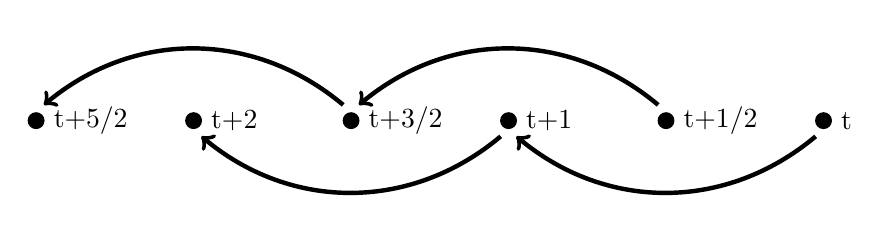
\begin{tikzpicture}[]
		\draw[<-,ultra thick] (0.1,0.2) to [out=40,in=140] (3.9,0.2);
		\draw[<-,ultra thick] (2.1,-0.2) to [out=-40,in=-140] (5.9,-0.2);
		\draw[<-,ultra thick] (4.1,0.2) to [out=40,in=140] (7.9,0.2);
		\draw[<-,ultra thick] (6.1,-0.2) to [out=-40,in=-140] (9.9,-0.2);
		\draw[fill] (0, 0) circle [radius=0.1];
		\draw[fill] (2, 0) circle [radius=0.1];
		\draw[fill] (4, 0) circle [radius=0.1];
		\draw[fill] (6, 0) circle [radius=0.1];
		\draw[fill] (8, 0) circle [radius=0.1];
		\draw[fill] (10, 0) circle [radius=0.1];
		\node [right] at (0.1,0) {t+5/2};
		\node [right] at (2.1,0) {t+2};
		\node [right] at (4.1,0) {t+3/2};
		\node [right] at (6.1,0) {t+1};
		\node [right] at (8.1,0) {t+1/2};
		\node [right] at (10.1,0) {t};	
		\end{tikzpicture}
	}
	\captionof{figure}{}
	\label{fig:time_grid}
	\end{minipage}
	And writing (\ref{eq:time_shift}) in the form
	\begin{align}
		\mathbf{r}^{t+1}_{n,m}=&\mathbf{T}(\mathbf{r}^t_{n,m};A^{t+1/2}_{n,m},B^{t+1/2}_{n,m}) \label{eq:leap_frog_shift_1} \\
		\mathbf{r}^{t+3/2}_{n,m}=&\mathbf{T}(\mathbf{r}^{t+1/2}_{n,m};A^{t+1}_{n,m},B^{t+1}_{n,m}) \label{eq:leap_frog_shift_2}
	\end{align}
	Use of these equations is indicated by lower and upper arrows in fig \ref{fig:time_grid}. To start this system we calculate $\mathbf{r}^{1/2}_{n,m}$ by using eq. (\ref{eq:time_shift}) and then shift to leap-frog method.
    \section{CUDA and CPU code}
    The above described numerical algorithm was implemented in C with 
    OpenMP \footnote{http://en.wikipedia.org/wiki/OpenMP} and in 
    C CUDA \footnote{http://en.wikipedia.org/wiki/OpenMP} and run on NVidia consumer grade GPGPU GTX680. 
    In this section we look at overall implementation of the code and compare two different approaches.
    \section{Results and Discussion}
    We assume that mini-band width $\Delta_1=60$ meV and SL period $d=6$ nm. Values close to these where engineered
    in the actual experiments. For example, in \cite{PhysRevB.56.10303} SL period is $3.8$ nm. and $\Delta_1=?$. 
    Thus, our values of $\Delta_1$ and $d$ represent middle of the road path easily accessible to the
    experimentalists. However, in our dimensionless form of Boltzmann equation, these parameters are encapsulated
    in parameter $\alpha$ (\ref{eq:alpha_def}), which takes value $\alpha=0.9496$, used throughout this work. 
    
    Looking at equations (\ref{eq:a_n_dot}) and (\ref{eq:b_n_dot}) we can branch out into several different 
    directions based on which of the external parameters $\tilde{B}$, $\tilde{E}_{dc}$ and $\tilde{E}_\omega$ 
    are zeroed and which are not. In this work we consider the most difficult case when all three parameters
    are not zero at non-zero temperature, but we will also look at the case where $\tilde{E}_\omega=0$, where
    correspondence between solutions of Boltzmann equation and classical pendulum can be most easily be seen.
    
    We will speak of space $(\phi_x,\phi_y)$ as a "phase space", since it is equivalent to the real phase space of 
    the classical pendulum $(\phi_x,\text{d}\phi_x/\text{d}t)$, caveat linear transformation between $\phi_x$ and 
    $\text{d}\phi_x/\text{d}t$ \ref{eq:semi_classical_phi_x_dot}. All of the figures in this work, showing electron 
    density function are presented in $(\phi_x,\phi_y)$ space, with $\phi_x$ alone the $x$-axis and $\phi_y$ along
    the $y$-axis. Electron density $f$ in the phase space $(\phi_x,\phi_y)$ spreads out, starting from Boltzmann 
    distribution, under the influence of electric and magnetic fields. Typical evolution of electron density function
    looks like this.
    \begin{figure}[H]
   	  \centering
	  \normalsize % use normal font size in the figure
	  \includegraphics[scale=0.5]{plots/example_of_time_evolution_of_f.pdf}
	  \label{fig:example_of_time_evolution_of_f}
	  \caption{$E_{dc}=7$ $E_\omega=0$ $\mu=11.6$ $\alpha=0.9496$ $B=4$}
	\end{figure}
	Where, you can see initial Boltzmann distribution shown on the frame 0 evolves through the transient 
	processes 1,2,3 and 4 into a final, "eye" like, state seen on frame 6.
	
    Depending on presence or absence
    of a/c emf, $E_\omega$, electron density function reaches either dynamic or static equilibrium. Videos of 
    time evolution of $f(\phi_x,\phi_y)$ for several different initial parameters, with a/c emf turned on, is
    available \footnote{\url{http://youtu.be/PMJSV7SSMlg}} \footnote{\url{http://youtu.be/FKYtk16-rVY}}. When 
    $E_{\omega}=0$, we can easily see clear correspondence between phase portraits of classical pendulum and
    electron density can be easily seen, as on the example below.
    \begin{figure}[H]
   	  \centering
	  \normalsize % use normal font size in the figure
	  \includegraphics[scale=0.45]{plots/classical_pendulum_phase_portrait_B_is_4_E_dc_is_6_point_5.pdf}
	  \label{fig:classical_and_boltzmann_correspondence_map}
	  \caption{$\tilde{B}=4$ $E_{dc}=6.5$ $\tilde{E}_{\omega}=0$ $\mu=5$ $\alpha=0.9496$}
	\end{figure}
	Important feature of these plots, is presence, in the phase portrait, of separatrix (shown in red), that separates
	"cyclotron-like" motion confined within separatrix and "Bloch-like" motion that lies outside of separatrix and 
	presence of the same pattern and two distinct regions in the portrait of electron density on the right. Note, that,
	assuming non-zero value of $\tilde{B}$, depending on value of $\tilde{E}_{dc}$ there are three possible regimes.
    \begin{figure}[H]
   	  \centering
	  \normalsize % use normal font size in the figure
	  \includegraphics[scale=0.3]{plots/three_types_of_f.pdf}
	  \label{fig:three_regimes}
	  \caption{$\tilde{B}=4$ $\tilde{E}_{\omega}=0$ $\mu=116$ $\alpha=0.9496$ 
	  and $E_{dc}$ is (a) 6, (b) 8, (c) 10. }
	\end{figure}
	Pure cyclotron regime seen in (a), mixed (b) and Bloch regime in (c). Note, that as temperature increase and
	distribution function spreads out, it is possible to transition from cyclotron to mixed regime. In this work, we
    always use value $\tilde{B} = 4$ and vary $\tilde{E}_{dc}$. 
    
    In the presence of a/c emf electron density does not reach a static state, but arrives to certain dynamic 
    equilibrium where it ”breathes” in or out of sync with external oscillations, giving us negative or positive
    (amplification) absorption. One of the simplest ways to think about negative absorption is to correlate it with
    negative effective mass, where electron in essence moves in the direction opposite of the applied force, thus 
    creating an equivalent of positive feedback loop, which is commonly used technique in signal amplification and
    generation. And indeed such amplifiers have been proposed in the past \cite{PhysRev.109.1856} and more recent 
    works considered concept of negative effective mass in order to understand dynamics of electrons in superlattices
    \cite{Gribnikov2002276}. However, negative effective mass is not actually necessary condition for negative absorption
    and later we show examples when effective mass is positive while absorption is negative.
    
    Another important parameter, that we look at is average drift velocity along the $\phi_x$ axis, which corresponds 
    to current flowing through the SL. Following plots link $\tilde{E}_{dc}$ and average drift velocity, i.e. 
    voltage-current characteristic.
   	\begin{figure}[H]
	  \centering
	  \normalsize % use normal font size in the figure
	  \includegraphics[scale=0.5]{plots/v_dr_and_m_vary_E_dc_and_mu.pdf}
	  \caption{$E_\omega=0.1$, $\omega=2.455$, $B=4$, $\alpha=0.9496$}
	  \label{fig:effect_of_temperature_in_v_dr_vary_E_dc_omega=2.455}	  
	\end{figure}	
	You can see that downward slope of drift velocity (shaded in light-red) closely corresponds to the negative effective
	mass (shared in light-blue), for low temperatures ($\mu = 216$, $\mu = 116$) and less so for higher 
	temperatures ($\mu = 11.6$ and $\mu = 1.16$ ). Similar correlation holds between negative absorption and effective
	mass in the next figure.
	\begin{figure}[H]
	  \centering
	  \normalsize % use normal font size in the figure
	  \includegraphics[scale=0.5]{plots/A_and_m_vary_E_dc_and_mu.pdf}
	  \caption{$E_\omega=0.1$, $\omega=2.455$, $B=4$, $\alpha=0.9496$, $\mu=[1.16, 11.6, 116, 216]$}
	  \label{fig:effect_of_temperature_in_A_vary_E_dc_omega=2.455}
	\end{figure}	
	For another value of $\omega$ situation is different. Correlation between downward slope of drift velocity and 
	negative effective mass still holds.
	\begin{figure}[H]
	  \centering
	  \normalsize % use normal font size in the figure
	  \includegraphics[scale=0.5]{plots/v_dr_and_m_vary_E_dc_and_mu_omega=4.pdf}
	  \caption{$\tilde{E}_\omega=0.1$, $\omega=4$, $\tilde{B}=4$, $\alpha=0.9496$}
	  \label{fig:effect_of_temperature_in_v_dr_vary_E_dc_omega=4}	  
	\end{figure}
	but not so much between absorption and negative effective mass
	\begin{figure}[H]
	  \centering
	  \normalsize % use normal font size in the figure
	  \includegraphics[scale=0.5]{plots/A_and_m_vary_E_dc_and_mu_omega=4.pdf}
	  \caption{$\tilde{E}_\omega=0.1$, $\omega=4$, $\tilde{B}=4$, $\alpha=0.9496$}
	  \label{fig:effect_of_temperature_in_A_vary_E_dc_omega=4}
	\end{figure}
	Here you can see region of negative absorption even though effective mass is positive. Following heat maps of
absorption and different parameters show that even better.
	\begin{figure}[H]
	  \centering
	  \normalsize % use normal font size in the figure
	  \includegraphics[scale=0.5]{plots/absorption_maps_E_omega_is_0_point_1_mu_is_116_alpha_0_point_0496.pdf}
	  \caption{Maps of absoprtion for $E_\omega=0.1$, $\alpha=0.9496$, $\mu=116$, $\tilde{B}=[1,3,4,8]$ 
	  (plots (a), (b), (c) and (d)) as a function of $\tilde{E}$ (on the x-axis) and $\omega$ (on the y-axis)}
	  \label{fig:absorption}	  
	\end{figure}
	In each heat-map type plot we have $E_{dc}$ along the $x$-axis and $\tilde{\omega}$ along the $y$-axis. 
	Dotted line show demarcation between positive and negative effective mass. To the right of it, effective map is
	negative, to the left positive. In figure (a) it is positive everywhere. Additionally, solid black line marks all
	points where $\Omega$ of the classical pendulum (74, 75) equals to $\tilde{\omega}$, frequency of external a/c emf.
	Red-to-yellow hues mark positive absorption and white to dark grey mark negative absorption. Separatrix of the
	classical pendulum is marked, by discontinuity of $\Omega$-lines. Important feature of these maps is clear present 
	of three distinct regions of negative absorption, especially clear present when temperature decreases 
	($\mu$ increases). One is cyclotron resonance to the left of the separatrix, Bloch resonance to right of the
	separatrix and region right around separatrix. The last one especially interesting because it show negative
	absorption both, at high temperatures (a) and at low frequency of a/c emf ( all maps ). We can look at map (c) in
	greater detail.
	\begin{figure}[H]
	  \centering
	  \normalsize % use normal font size in the figure
	  \includegraphics[scale=0.5]{plots/B=4_map_and_3_A_and_Asin_plots.pdf}
	  \caption{For map of absorption (a) for $\tilde{B}=4$ we are looking at just the crossections of the
	  map showing absorption $A$ and $ASIN$ components as a functions of $\omega$ at three different values of $E_{dc}$.
	  Plot (b) corresponds to $E_{dc}=6.5$, (c) $E_{dc}=8.2$ and (d) $E_{dc}=9.5$. Line (e) corresponds to $E_{dc}=7.8$, 
	  below you will find figure \ref{fig:E_dc=7.8_B=4_different_mu} that corresponds to this line. Line (f) 
	  corresponds to $E_{dc}=7.0$, below you will find figure \ref{fig:E_dc=7.0_B=4_different_mu} that corresponds to this line.}
	  \label{fig:map_of_absorption_and_profiles_for_three_different_E_dc_B=4}
	\end{figure}
	Now we are going to look at the plots absorption and dispersion (ASIN) for the same lines (b), (c), (d), (e) and (f)
for several different values of $\mu$ slowly rising temperature. While we expect, in general, rising temperature, to have
smoothing effect on these plots as electron collisions with the lattice starts having dominating effect over everything
else, we will some odd effects. You can see that on the very next figure that corresponds to plot (b) above.
	\begin{figure}[H]
	  \centering
	  \normalsize % use normal font size in the figure
	  \includegraphics[scale=0.35]{plots/A_and_ASIN_of_omega_E_dc_is_6_point_5_vary_mu.pdf}
	  \caption{This shows effect of raising temperature on absorption and ASIN as functions of $\omega$ for 
	  parameters that correspond to Fig \ref{fig:map_of_absorption_and_profiles_for_three_different_E_dc_B=4}(b)}
	  \label{fig:E_dc=6.5_B=4_different_mu}	  
	\end{figure}
	You can see here that as temperature rises ($\mu$ goes down), so lowers absorption at $\tilde{\omega} = 0.5$ and
	at $\mu = 3$ crosses into negative region before rising again to 0 at $\mu = 1.16$. This effect is even more
	pronounced for Fig. \ref{fig:map_of_absorption_and_profiles_for_three_different_E_dc_B=4}(f)
	\begin{figure}[H]
	  \centering
	  \normalsize % use normal font size in the figure
	  \includegraphics[scale=0.35]{plots/A_and_ASIN_of_omega_E_dc_is_7_point_0_vary_mu.pdf}
	  \caption{This shows effect of raising temperature on absorption and ASIN as functions of $\omega$ for 
	  parameters that correspond to Fig \ref{fig:map_of_absorption_and_profiles_for_three_different_E_dc_B=4}(f)}
	  \label{fig:E_dc=7.0_B=4_different_mu}	  
	\end{figure}
    where you can see that absorption becomes negative for $\tilde{\omega} = 0.5$ already at $\mu = 32.16$. This effect
    can be attributed to the fact that at these parameters and low temperature electron distribution packet is contained
    within the Brillouin zone in cyclotron mode, and rising temperature spreads the packet until it crosses separatix and
    enters into Bloch regime. This process could, in principle, allow signal amplification even at room temperatures.
    What will be important is to find right parameters for the actual semiconductor super lattice, so that we would be
    sitting right around line (f) in figure \ref{fig:map_of_absorption_and_profiles_for_three_different_E_dc_B=4}.

    However, once we come very close to separatrix $E_{dc} = 7.8$ and then cross it $E_{dc} > 8$ then suppression of
    absorption with rising temperatures becomes much simpler as you can see in the next three figures.
	\begin{figure}[H]
	  \centering
	  \normalsize % use normal font size in the figure
	  \includegraphics[scale=0.35]{plots/A_and_ASIN_of_omega_E_dc_is_7_point_8_vary_mu.pdf}
	  \caption{This shows effect of raising temperature on absorption and ASIN as functions of $\omega$ for parameters
	  that correspond to Fig \ref{fig:map_of_absorption_and_profiles_for_three_different_E_dc_B=4}(e)}
	  \label{fig:E_dc=7.8_B=4_different_mu}	  
	\end{figure}
	Notable in this figure and the next one, both of which corresponds to regime right around separatrix, that negative
	absorption is preserved even as temperature rises essentially to room temperature $\mu = 1.16$. However, stability of
	amplification of around separatix is questionable since corresponding classical pendulum is known to exhibit chaos in
	this regime.
	\begin{figure}[H]
	  \centering
	  \normalsize % use normal font size in the figure
	  \includegraphics[scale=0.35]{plots/A_and_ASIN_of_omega_E_dc_is_8_point_2_vary_mu.pdf}
	  \caption{This shows effect of raising temperature on absorption and ASIN as functions of $\omega$ for parameters 
	  that correspond to Fig \ref{fig:map_of_absorption_and_profiles_for_three_different_E_dc_B=4}(c)}
	  \label{fig:E_dc=8.2_B=4_different_mu}
	\end{figure}
	\begin{figure}[H]
	  \centering
	  \normalsize % use normal font size in the figure
	  \includegraphics[scale=0.35]{plots/A_and_ASIN_of_omega_E_dc_is_9_point_5_vary_mu.pdf}
	  \caption{This shows effect of raising temperature on absorption and ASIN as functions of $\omega$ for parameters 
	  that correspond to Fig \ref{fig:map_of_absorption_and_profiles_for_three_different_E_dc_B=4}(d)}
	  \label{fig:E_dc=9.5_B=4_different_mu}	  
	\end{figure}
    One of the way that we can use to understand signal absorption and amplification in SL is to consider formation
    of bunches in $k$-space. In vacuum electronics this effect is known as bunching and can be studied in both, real and
    momentum spaces. In our case visualization of bunches in momentum space would require, hard to understand and
    visualize, electron density plot in three dimensions $f(\phi_x, \phi_y, t)$. To make that task more manageable we
    reduce dimensionality of $f$ through integration
    \begin{equation}
        f(\phi_x,t)=\int^{\infty}_{-\infty}f(\phi_x,\phi_y,t)\text{d}\phi_x
    \end{equation}
    We correlate this heat-map plot with drift velocity and a/c component of external field. Note that, instead of time 
    $t$ we use $\tilde{\omega}t$. First we look at case of strong negative absorption at $\tilde{\omega} = 2.455$ that
    corresponds to local a minimum, a blue line ($\mu = 116$) in figure \ref{fig:E_dc=7.8_B=4_different_mu}. At the
    bottom of the plot you see external a/c emf component time evolution shown as black line, also overlaid as a white
    live over the main part of distribution function, and the drift velocity as a function of time is shown at the bottom
    section in red. Both $v_{dr}$ and a/c emf component are scaled to be comparable to each other, so that we can easily
    compare them.
	\begin{figure}[H]
	  \centering
	  \normalsize % use normal font size in the figure
	  \includegraphics[scale=0.5]{plots/bunching_2_point_455.pdf}
	  \caption{}	  
	\end{figure}
	Both $v_{dr}$ and a/c emf component are scaled to be comparable to each other, so that we can easily compare them.
	You can see that they, $v_{dr}$ and a/c emf, are almost completely out of phase, giving rise to strong negative
	absorption. It is also easy to see bunches in $k$-space (or $\phi$-space in our case ) at the bottom of the density
	map. It	is important to note that presence of electron density in negative region of $\phi_x$ is due to the magnetic
	field wrapping $f(\phi_x; \phi_y)$ and not to crossing of the Brillouin zone boundaries. To better see bunching in
	the positive region of $\phi_x$ we need to zoom in, result of which is shown in the next figure.
	\begin{figure}[H]
	  \centering
	  \normalsize % use normal font size in the figure
	  \includegraphics[scale=0.5]{plots/bunching_2_point_455_zoom.pdf}
	  \caption{}	  
	\end{figure}
	\newpage
    A similar map can be plotted for a case of strong positive absorption.
	\begin{figure}[H]
	  \centering
	  \normalsize % use normal font size in the figure
	  \includegraphics[scale=0.5]{plots/bunching_5_point_1.pdf}
	  \caption{}	  
	\end{figure}
	which corresponds to the local maximum of absorption at $\tilde{\omega} = 2.455$, a blue line ($\mu = 116$) 
	in figure \ref{fig:E_dc=7.8_B=4_different_mu}. And zooming of this map.
	\begin{figure}[H]
	  \centering
	  \normalsize % use normal font size in the figure
	  \includegraphics[scale=0.5]{plots/bunching_5_point_1_zoom.pdf}
	  \caption{}	  
	\end{figure}    
	Here you can see similar bunches formed in the k-space, but $v_{dr}$ (red line) as function of time is almost
    completely in phase with external a/c emf (black line).
    \section{Conclusions}
    We predicted two small signal amplification regimes that differ from widely discussed Bloch gain regime. One is for
    high frequency signal when SL operates in cyclotron regime, which mainly manifest at low temperatures. And another
    is one for low frequency signal when, for a narrow set of parameters, electron distribution slightly overflows over
    the edge of the Brillouin zone. This research can be extended in several directions. One, is farther theoretical
    study of SL in presence of magnetic field. Specifically, study of stability of amplification, especially around
    separatix. Also, it is important to look at the case where spacial homogeneity is not assumed and verify that
    electron bunching in real space does not occur or if it does that it is does not destroy picture of small signal
    amplification presented in this paper. Strong signal amplification should also be considered as it should expose
    nonlinearity of dispersion relation even more and is a very interesting topic to consider. On experimental front,
    verification of our findings would be most welcome.    
  	\bibliography{master}
   	\newpage
    \section{Additional figures}
	\begin{figure}[H]
	  \centering
	  \normalsize
	  % GNUPLOT: LaTeX picture with Postscript
\begingroup
  \makeatletter
  \providecommand\color[2][]{%
    \GenericError{(gnuplot) \space\space\space\@spaces}{%
      Package color not loaded in conjunction with
      terminal option `colourtext'%
    }{See the gnuplot documentation for explanation.%
    }{Either use 'blacktext' in gnuplot or load the package
      color.sty in LaTeX.}%
    \renewcommand\color[2][]{}%
  }%
  \providecommand\includegraphics[2][]{%
    \GenericError{(gnuplot) \space\space\space\@spaces}{%
      Package graphicx or graphics not loaded%
    }{See the gnuplot documentation for explanation.%
    }{The gnuplot epslatex terminal needs graphicx.sty or graphics.sty.}%
    \renewcommand\includegraphics[2][]{}%
  }%
  \providecommand\rotatebox[2]{#2}%
  \@ifundefined{ifGPcolor}{%
    \newif\ifGPcolor
    \GPcolortrue
  }{}%
  \@ifundefined{ifGPblacktext}{%
    \newif\ifGPblacktext
    \GPblacktextfalse
  }{}%
  % define a \g@addto@macro without @ in the name:
  \let\gplgaddtomacro\g@addto@macro
  % define empty templates for all commands taking text:
  \gdef\gplbacktext{}%
  \gdef\gplfronttext{}%
  \makeatother
  \ifGPblacktext
    % no textcolor at all
    \def\colorrgb#1{}%
    \def\colorgray#1{}%
  \else
    % gray or color?
    \ifGPcolor
      \def\colorrgb#1{\color[rgb]{#1}}%
      \def\colorgray#1{\color[gray]{#1}}%
      \expandafter\def\csname LTw\endcsname{\color{white}}%
      \expandafter\def\csname LTb\endcsname{\color{black}}%
      \expandafter\def\csname LTa\endcsname{\color{black}}%
      \expandafter\def\csname LT0\endcsname{\color[rgb]{1,0,0}}%
      \expandafter\def\csname LT1\endcsname{\color[rgb]{0,1,0}}%
      \expandafter\def\csname LT2\endcsname{\color[rgb]{0,0,1}}%
      \expandafter\def\csname LT3\endcsname{\color[rgb]{1,0,1}}%
      \expandafter\def\csname LT4\endcsname{\color[rgb]{0,1,1}}%
      \expandafter\def\csname LT5\endcsname{\color[rgb]{1,1,0}}%
      \expandafter\def\csname LT6\endcsname{\color[rgb]{0,0,0}}%
      \expandafter\def\csname LT7\endcsname{\color[rgb]{1,0.3,0}}%
      \expandafter\def\csname LT8\endcsname{\color[rgb]{0.5,0.5,0.5}}%
    \else
      % gray
      \def\colorrgb#1{\color{black}}%
      \def\colorgray#1{\color[gray]{#1}}%
      \expandafter\def\csname LTw\endcsname{\color{white}}%
      \expandafter\def\csname LTb\endcsname{\color{black}}%
      \expandafter\def\csname LTa\endcsname{\color{black}}%
      \expandafter\def\csname LT0\endcsname{\color{black}}%
      \expandafter\def\csname LT1\endcsname{\color{black}}%
      \expandafter\def\csname LT2\endcsname{\color{black}}%
      \expandafter\def\csname LT3\endcsname{\color{black}}%
      \expandafter\def\csname LT4\endcsname{\color{black}}%
      \expandafter\def\csname LT5\endcsname{\color{black}}%
      \expandafter\def\csname LT6\endcsname{\color{black}}%
      \expandafter\def\csname LT7\endcsname{\color{black}}%
      \expandafter\def\csname LT8\endcsname{\color{black}}%
    \fi
  \fi
  \setlength{\unitlength}{0.0500bp}%
  \begin{picture}(10080.00,6048.00)%
    \gplgaddtomacro\gplbacktext{%
      \csname LTb\endcsname%
      \put(688,512){\makebox(0,0)[r]{\strut{} 0}}%
      \csname LTb\endcsname%
      \put(688,1018){\makebox(0,0)[r]{\strut{} 0.1}}%
      \csname LTb\endcsname%
      \put(688,1523){\makebox(0,0)[r]{\strut{} 0.2}}%
      \csname LTb\endcsname%
      \put(688,2029){\makebox(0,0)[r]{\strut{} 0.3}}%
      \csname LTb\endcsname%
      \put(688,2534){\makebox(0,0)[r]{\strut{} 0.4}}%
      \csname LTb\endcsname%
      \put(688,3040){\makebox(0,0)[r]{\strut{} 0.5}}%
      \csname LTb\endcsname%
      \put(688,3545){\makebox(0,0)[r]{\strut{} 0.6}}%
      \csname LTb\endcsname%
      \put(688,4051){\makebox(0,0)[r]{\strut{} 0.7}}%
      \csname LTb\endcsname%
      \put(688,4556){\makebox(0,0)[r]{\strut{} 0.8}}%
      \csname LTb\endcsname%
      \put(688,5062){\makebox(0,0)[r]{\strut{} 0.9}}%
      \csname LTb\endcsname%
      \put(688,5567){\makebox(0,0)[r]{\strut{} 1}}%
      \csname LTb\endcsname%
      \put(784,352){\makebox(0,0){\strut{} 0}}%
      \csname LTb\endcsname%
      \put(2285,352){\makebox(0,0){\strut{} 2}}%
      \csname LTb\endcsname%
      \put(3786,352){\makebox(0,0){\strut{} 4}}%
      \csname LTb\endcsname%
      \put(5287,352){\makebox(0,0){\strut{} 6}}%
      \csname LTb\endcsname%
      \put(6788,352){\makebox(0,0){\strut{} 8}}%
      \csname LTb\endcsname%
      \put(8289,352){\makebox(0,0){\strut{} 10}}%
      \csname LTb\endcsname%
      \put(9790,352){\makebox(0,0){\strut{} 12}}%
      \put(128,3039){\rotatebox{-270}{\makebox(0,0){\strut{}$v_{dr}/v_{p}$}}}%
      \put(5287,112){\makebox(0,0){\strut{}$E_{dc}/E_{*}$}}%
      \put(5287,5807){\makebox(0,0){\strut{}$v_{dr}/v_{p}=f(E_{dc}/E_{*})$ $\mu=[1.16, 11.6, 116, 232]$ $\alpha=0.9496$ $B=4$ $E_{\omega}=0$}}%
    }%
    \gplgaddtomacro\gplfronttext{%
      \csname LTb\endcsname%
      \put(9055,5424){\makebox(0,0)[r]{\strut{}$\mu=232$}}%
      \csname LTb\endcsname%
      \put(9055,5264){\makebox(0,0)[r]{\strut{}$\mu=116$}}%
      \csname LTb\endcsname%
      \put(9055,5104){\makebox(0,0)[r]{\strut{}$\mu=11.6$}}%
      \csname LTb\endcsname%
      \put(9055,4944){\makebox(0,0)[r]{\strut{}$\mu=1.16$}}%
      \csname LTb\endcsname%
      \put(9055,4784){\makebox(0,0)[r]{\strut{}B=0 Esaki-Tsu}}%
    }%
    \gplbacktext
    \put(0,0){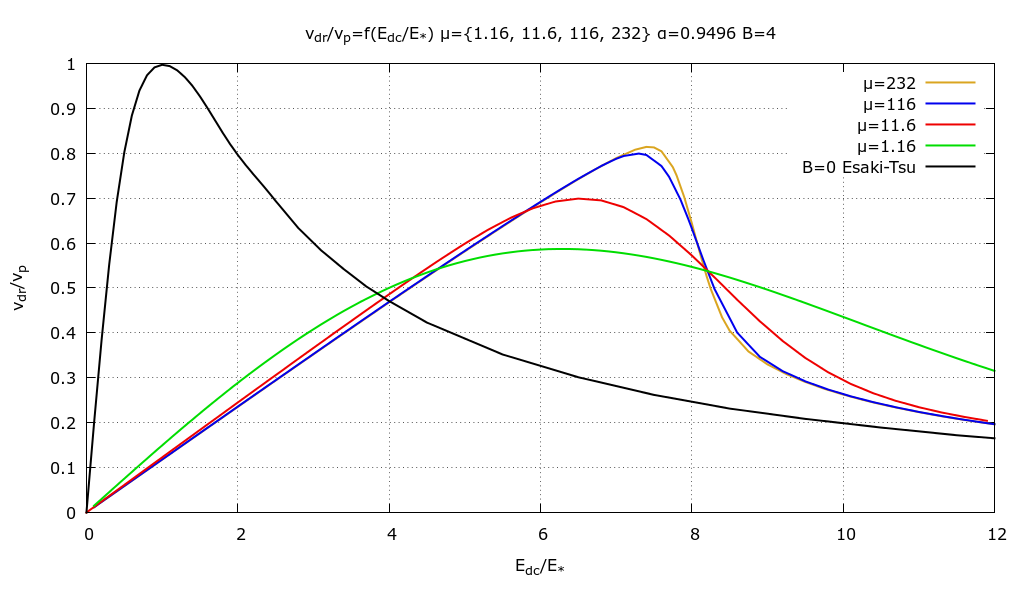
\includegraphics{v_dr_of_e_dc_B=4_mu=11_dot_6_116}}%
    \gplfronttext
  \end{picture}%
\endgroup

	  \label{fig:v_dr_of_E_dc_B=4_different_mu}
	  \caption{Here we are looking at effect of rising temperature of, essentially, voltage to current characteristic,
	  since current is proportional to $v_{dr}$, which is along the $y$-axis and voltage across SL is proportional to 
	  $E_{dc}$, which is along the $x$-axis. Also, a/a component is is not present, $E_{\omega} = 0$. For reference we
	  show Esaki-Tsu characteristic, which correspond to absence of magnetic field, analytical expression for which
	  is well known. You can see that as temperature lowers ($\mu$ rises) $v_{dr}$ as a function of $E_{dc}$ behaves
	  more and more linearly for $E_{dc} < 7$ and undergoes sudden step-like drop around $E_{dc} = 8$. Rising temperature
	  (lowering $\mu$), naturally, removes the step and smoothes whole plot.}
	\end{figure}
	\newpage
	\begin{figure}[H]
	  \centering
	  \normalsize
	  % GNUPLOT: LaTeX picture with Postscript
\begingroup
  \makeatletter
  \providecommand\color[2][]{%
    \GenericError{(gnuplot) \space\space\space\@spaces}{%
      Package color not loaded in conjunction with
      terminal option `colourtext'%
    }{See the gnuplot documentation for explanation.%
    }{Either use 'blacktext' in gnuplot or load the package
      color.sty in LaTeX.}%
    \renewcommand\color[2][]{}%
  }%
  \providecommand\includegraphics[2][]{%
    \GenericError{(gnuplot) \space\space\space\@spaces}{%
      Package graphicx or graphics not loaded%
    }{See the gnuplot documentation for explanation.%
    }{The gnuplot epslatex terminal needs graphicx.sty or graphics.sty.}%
    \renewcommand\includegraphics[2][]{}%
  }%
  \providecommand\rotatebox[2]{#2}%
  \@ifundefined{ifGPcolor}{%
    \newif\ifGPcolor
    \GPcolortrue
  }{}%
  \@ifundefined{ifGPblacktext}{%
    \newif\ifGPblacktext
    \GPblacktextfalse
  }{}%
  % define a \g@addto@macro without @ in the name:
  \let\gplgaddtomacro\g@addto@macro
  % define empty templates for all commands taking text:
  \gdef\gplbacktext{}%
  \gdef\gplfronttext{}%
  \makeatother
  \ifGPblacktext
    % no textcolor at all
    \def\colorrgb#1{}%
    \def\colorgray#1{}%
  \else
    % gray or color?
    \ifGPcolor
      \def\colorrgb#1{\color[rgb]{#1}}%
      \def\colorgray#1{\color[gray]{#1}}%
      \expandafter\def\csname LTw\endcsname{\color{white}}%
      \expandafter\def\csname LTb\endcsname{\color{black}}%
      \expandafter\def\csname LTa\endcsname{\color{black}}%
      \expandafter\def\csname LT0\endcsname{\color[rgb]{1,0,0}}%
      \expandafter\def\csname LT1\endcsname{\color[rgb]{0,1,0}}%
      \expandafter\def\csname LT2\endcsname{\color[rgb]{0,0,1}}%
      \expandafter\def\csname LT3\endcsname{\color[rgb]{1,0,1}}%
      \expandafter\def\csname LT4\endcsname{\color[rgb]{0,1,1}}%
      \expandafter\def\csname LT5\endcsname{\color[rgb]{1,1,0}}%
      \expandafter\def\csname LT6\endcsname{\color[rgb]{0,0,0}}%
      \expandafter\def\csname LT7\endcsname{\color[rgb]{1,0.3,0}}%
      \expandafter\def\csname LT8\endcsname{\color[rgb]{0.5,0.5,0.5}}%
    \else
      % gray
      \def\colorrgb#1{\color{black}}%
      \def\colorgray#1{\color[gray]{#1}}%
      \expandafter\def\csname LTw\endcsname{\color{white}}%
      \expandafter\def\csname LTb\endcsname{\color{black}}%
      \expandafter\def\csname LTa\endcsname{\color{black}}%
      \expandafter\def\csname LT0\endcsname{\color{black}}%
      \expandafter\def\csname LT1\endcsname{\color{black}}%
      \expandafter\def\csname LT2\endcsname{\color{black}}%
      \expandafter\def\csname LT3\endcsname{\color{black}}%
      \expandafter\def\csname LT4\endcsname{\color{black}}%
      \expandafter\def\csname LT5\endcsname{\color{black}}%
      \expandafter\def\csname LT6\endcsname{\color{black}}%
      \expandafter\def\csname LT7\endcsname{\color{black}}%
      \expandafter\def\csname LT8\endcsname{\color{black}}%
    \fi
  \fi
  \setlength{\unitlength}{0.0500bp}%
  \begin{picture}(10080.00,6048.00)%
    \gplgaddtomacro\gplbacktext{%
      \csname LTb\endcsname%
      \put(688,512){\makebox(0,0)[r]{\strut{}-0.4}}%
      \csname LTb\endcsname%
      \put(688,1186){\makebox(0,0)[r]{\strut{}-0.2}}%
      \csname LTb\endcsname%
      \put(688,1860){\makebox(0,0)[r]{\strut{} 0}}%
      \csname LTb\endcsname%
      \put(688,2534){\makebox(0,0)[r]{\strut{} 0.2}}%
      \csname LTb\endcsname%
      \put(688,3208){\makebox(0,0)[r]{\strut{} 0.4}}%
      \csname LTb\endcsname%
      \put(688,3882){\makebox(0,0)[r]{\strut{} 0.6}}%
      \csname LTb\endcsname%
      \put(688,4556){\makebox(0,0)[r]{\strut{} 0.8}}%
      \csname LTb\endcsname%
      \put(688,5230){\makebox(0,0)[r]{\strut{} 1}}%
      \csname LTb\endcsname%
      \put(784,352){\makebox(0,0){\strut{} 0}}%
      \csname LTb\endcsname%
      \put(2285,352){\makebox(0,0){\strut{} 2}}%
      \csname LTb\endcsname%
      \put(3786,352){\makebox(0,0){\strut{} 4}}%
      \csname LTb\endcsname%
      \put(5287,352){\makebox(0,0){\strut{} 6}}%
      \csname LTb\endcsname%
      \put(6788,352){\makebox(0,0){\strut{} 8}}%
      \csname LTb\endcsname%
      \put(8289,352){\makebox(0,0){\strut{} 10}}%
      \csname LTb\endcsname%
      \put(9790,352){\makebox(0,0){\strut{} 12}}%
      \put(128,3039){\rotatebox{-270}{\makebox(0,0){\strut{}$m/m_{x,k}$}}}%
      \put(5287,112){\makebox(0,0){\strut{}$E_{dc}/E_{*}$}}%
      \put(5287,5807){\makebox(0,0){\strut{}$m/m_{x,k}=f(E_{dc}/E_{*})$ $\mu=[1.16, 11.6, 116, 232]$ $\alpha=0.9496$ $B=4$ $E_{\omega}=0$}}%
    }%
    \gplgaddtomacro\gplfronttext{%
      \csname LTb\endcsname%
      \put(9055,5424){\makebox(0,0)[r]{\strut{}$\mu=232$}}%
      \csname LTb\endcsname%
      \put(9055,5264){\makebox(0,0)[r]{\strut{}$\mu=116$}}%
      \csname LTb\endcsname%
      \put(9055,5104){\makebox(0,0)[r]{\strut{}$\mu=11.6$}}%
      \csname LTb\endcsname%
      \put(9055,4944){\makebox(0,0)[r]{\strut{}$\mu=1.16$}}%
      \csname LTb\endcsname%
      \put(9055,4784){\makebox(0,0)[r]{\strut{}$\mu=116 B=0$}}%
    }%
    \gplbacktext
    \put(0,0){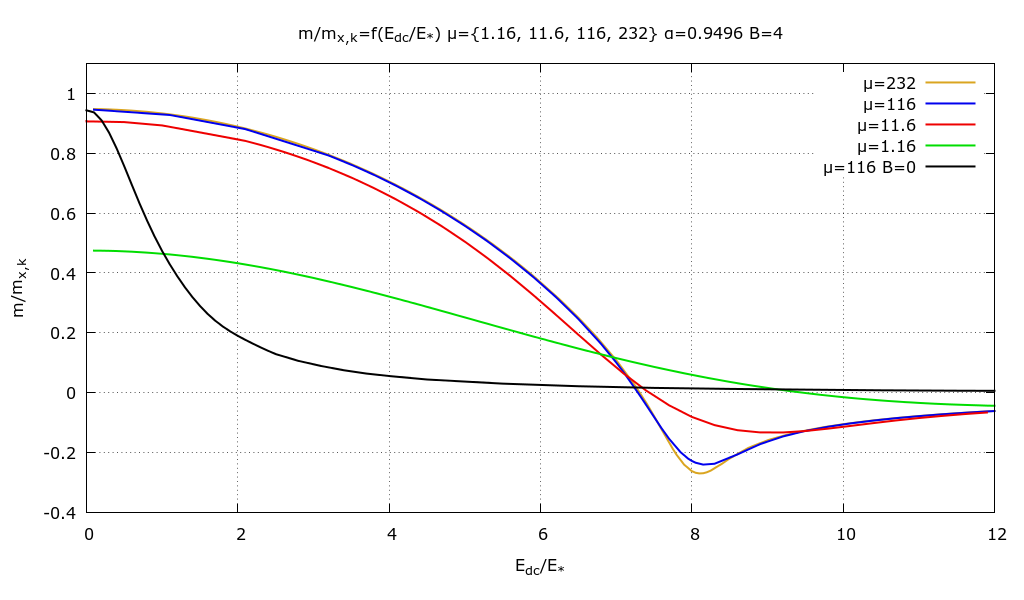
\includegraphics{m_over_m_xk_of_e_dc_B=4_mu=11_dot_6_116}}%
    \gplfronttext
  \end{picture}%
\endgroup

	  \label{fig:effect1ive_mass_of_E_dc_B=4_different_mu}
	  \caption{Here we are looking affective mass as a function of $E_{dc}$, that correspond to the previous figure. 
	  You can see that when slope of $v_{dr} = f(E_{dc})$ becomes negative effective mass becomes negative as well. 
	  For reference, case of B = 0 is drawn as black line showing positive effective mass everywhere.}
	\end{figure}
	\newpage
	\begin{figure}[H]
	  \centering
	  \normalsize % use normal font size in the figure
	  % GNUPLOT: LaTeX picture with Postscript
\begingroup
  \makeatletter
  \providecommand\color[2][]{%
    \GenericError{(gnuplot) \space\space\space\@spaces}{%
      Package color not loaded in conjunction with
      terminal option `colourtext'%
    }{See the gnuplot documentation for explanation.%
    }{Either use 'blacktext' in gnuplot or load the package
      color.sty in LaTeX.}%
    \renewcommand\color[2][]{}%
  }%
  \providecommand\includegraphics[2][]{%
    \GenericError{(gnuplot) \space\space\space\@spaces}{%
      Package graphicx or graphics not loaded%
    }{See the gnuplot documentation for explanation.%
    }{The gnuplot epslatex terminal needs graphicx.sty or graphics.sty.}%
    \renewcommand\includegraphics[2][]{}%
  }%
  \providecommand\rotatebox[2]{#2}%
  \@ifundefined{ifGPcolor}{%
    \newif\ifGPcolor
    \GPcolortrue
  }{}%
  \@ifundefined{ifGPblacktext}{%
    \newif\ifGPblacktext
    \GPblacktextfalse
  }{}%
  % define a \g@addto@macro without @ in the name:
  \let\gplgaddtomacro\g@addto@macro
  % define empty templates for all commands taking text:
  \gdef\gplbacktext{}%
  \gdef\gplfronttext{}%
  \makeatother
  \ifGPblacktext
    % no textcolor at all
    \def\colorrgb#1{}%
    \def\colorgray#1{}%
  \else
    % gray or color?
    \ifGPcolor
      \def\colorrgb#1{\color[rgb]{#1}}%
      \def\colorgray#1{\color[gray]{#1}}%
      \expandafter\def\csname LTw\endcsname{\color{white}}%
      \expandafter\def\csname LTb\endcsname{\color{black}}%
      \expandafter\def\csname LTa\endcsname{\color{black}}%
      \expandafter\def\csname LT0\endcsname{\color[rgb]{1,0,0}}%
      \expandafter\def\csname LT1\endcsname{\color[rgb]{0,1,0}}%
      \expandafter\def\csname LT2\endcsname{\color[rgb]{0,0,1}}%
      \expandafter\def\csname LT3\endcsname{\color[rgb]{1,0,1}}%
      \expandafter\def\csname LT4\endcsname{\color[rgb]{0,1,1}}%
      \expandafter\def\csname LT5\endcsname{\color[rgb]{1,1,0}}%
      \expandafter\def\csname LT6\endcsname{\color[rgb]{0,0,0}}%
      \expandafter\def\csname LT7\endcsname{\color[rgb]{1,0.3,0}}%
      \expandafter\def\csname LT8\endcsname{\color[rgb]{0.5,0.5,0.5}}%
    \else
      % gray
      \def\colorrgb#1{\color{black}}%
      \def\colorgray#1{\color[gray]{#1}}%
      \expandafter\def\csname LTw\endcsname{\color{white}}%
      \expandafter\def\csname LTb\endcsname{\color{black}}%
      \expandafter\def\csname LTa\endcsname{\color{black}}%
      \expandafter\def\csname LT0\endcsname{\color{black}}%
      \expandafter\def\csname LT1\endcsname{\color{black}}%
      \expandafter\def\csname LT2\endcsname{\color{black}}%
      \expandafter\def\csname LT3\endcsname{\color{black}}%
      \expandafter\def\csname LT4\endcsname{\color{black}}%
      \expandafter\def\csname LT5\endcsname{\color{black}}%
      \expandafter\def\csname LT6\endcsname{\color{black}}%
      \expandafter\def\csname LT7\endcsname{\color{black}}%
      \expandafter\def\csname LT8\endcsname{\color{black}}%
    \fi
  \fi
  \setlength{\unitlength}{0.0500bp}%
  \begin{picture}(10080.00,6048.00)%
    \gplgaddtomacro\gplbacktext{%
      \csname LTb\endcsname%
      \put(688,512){\makebox(0,0)[r]{\strut{} 0}}%
      \csname LTb\endcsname%
      \put(688,1018){\makebox(0,0)[r]{\strut{} 0.1}}%
      \csname LTb\endcsname%
      \put(688,1523){\makebox(0,0)[r]{\strut{} 0.2}}%
      \csname LTb\endcsname%
      \put(688,2029){\makebox(0,0)[r]{\strut{} 0.3}}%
      \csname LTb\endcsname%
      \put(688,2534){\makebox(0,0)[r]{\strut{} 0.4}}%
      \csname LTb\endcsname%
      \put(688,3040){\makebox(0,0)[r]{\strut{} 0.5}}%
      \csname LTb\endcsname%
      \put(688,3545){\makebox(0,0)[r]{\strut{} 0.6}}%
      \csname LTb\endcsname%
      \put(688,4051){\makebox(0,0)[r]{\strut{} 0.7}}%
      \csname LTb\endcsname%
      \put(688,4556){\makebox(0,0)[r]{\strut{} 0.8}}%
      \csname LTb\endcsname%
      \put(688,5062){\makebox(0,0)[r]{\strut{} 0.9}}%
      \csname LTb\endcsname%
      \put(688,5567){\makebox(0,0)[r]{\strut{} 1}}%
      \csname LTb\endcsname%
      \put(784,352){\makebox(0,0){\strut{} 0}}%
      \csname LTb\endcsname%
      \put(1763,352){\makebox(0,0){\strut{} 2}}%
      \csname LTb\endcsname%
      \put(2742,352){\makebox(0,0){\strut{} 4}}%
      \csname LTb\endcsname%
      \put(3721,352){\makebox(0,0){\strut{} 6}}%
      \csname LTb\endcsname%
      \put(4700,352){\makebox(0,0){\strut{} 8}}%
      \csname LTb\endcsname%
      \put(5679,352){\makebox(0,0){\strut{} 10}}%
      \csname LTb\endcsname%
      \put(6657,352){\makebox(0,0){\strut{} 12}}%
      \csname LTb\endcsname%
      \put(7636,352){\makebox(0,0){\strut{} 14}}%
      \csname LTb\endcsname%
      \put(8615,352){\makebox(0,0){\strut{} 16}}%
      \csname LTb\endcsname%
      \put(9594,352){\makebox(0,0){\strut{} 18}}%
      \put(128,3039){\rotatebox{-270}{\makebox(0,0){\strut{}$v_{dr}/v_{p}$}}}%
      \put(5287,112){\makebox(0,0){\strut{}$E_{dc}/E_{*}$}}%
      \put(5287,5807){\makebox(0,0){\strut{}$v_{dr}/v_{p}=f(E_{dc}/E_{*})$ $\mu=116$ $\alpha=0.9496$ $B=[0, 4, 8]$ $E_{\omega}=0$}}%
    }%
    \gplgaddtomacro\gplfronttext{%
      \csname LTb\endcsname%
      \put(9055,5424){\makebox(0,0)[r]{\strut{}B=8}}%
      \csname LTb\endcsname%
      \put(9055,5264){\makebox(0,0)[r]{\strut{}B=4}}%
      \csname LTb\endcsname%
      \put(9055,5104){\makebox(0,0)[r]{\strut{}B=0 Esaki-Tsu}}%
    }%
    \gplbacktext
    \put(0,0){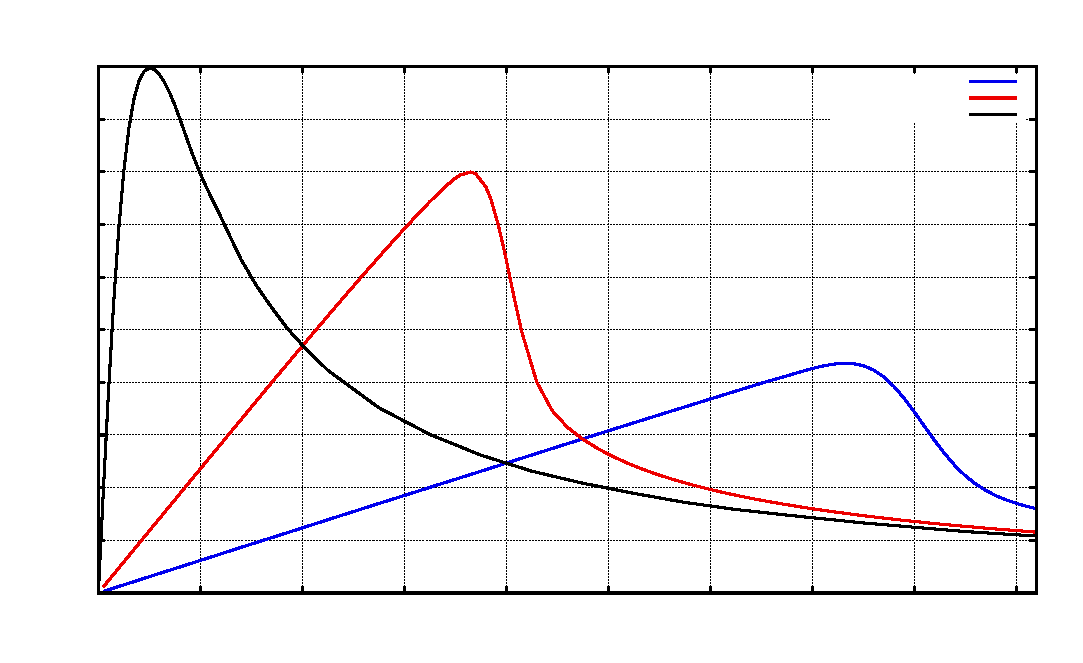
\includegraphics{v_dr_of_e_dc_B=diff}}%
    \gplfronttext
  \end{picture}%
\endgroup

	  \label{fig:v_dr_of_E_dc_different_B}
	  \caption{Here, again, we do not have a/c emf ($E_{dc} = 0$) are looking at how increasing strength of magnetic field
affects voltage-current characteristic. Temperature here is very low, $\mu = 116$, which roughly corresponds 
to 3 Kelvin.}
	\end{figure}
	\newpage
	\begin{figure}[H]
	  \centering
	  \normalsize % use normal font size in the figure
	  % GNUPLOT: LaTeX picture with Postscript
\begingroup
  \makeatletter
  \providecommand\color[2][]{%
    \GenericError{(gnuplot) \space\space\space\@spaces}{%
      Package color not loaded in conjunction with
      terminal option `colourtext'%
    }{See the gnuplot documentation for explanation.%
    }{Either use 'blacktext' in gnuplot or load the package
      color.sty in LaTeX.}%
    \renewcommand\color[2][]{}%
  }%
  \providecommand\includegraphics[2][]{%
    \GenericError{(gnuplot) \space\space\space\@spaces}{%
      Package graphicx or graphics not loaded%
    }{See the gnuplot documentation for explanation.%
    }{The gnuplot epslatex terminal needs graphicx.sty or graphics.sty.}%
    \renewcommand\includegraphics[2][]{}%
  }%
  \providecommand\rotatebox[2]{#2}%
  \@ifundefined{ifGPcolor}{%
    \newif\ifGPcolor
    \GPcolortrue
  }{}%
  \@ifundefined{ifGPblacktext}{%
    \newif\ifGPblacktext
    \GPblacktextfalse
  }{}%
  % define a \g@addto@macro without @ in the name:
  \let\gplgaddtomacro\g@addto@macro
  % define empty templates for all commands taking text:
  \gdef\gplbacktext{}%
  \gdef\gplfronttext{}%
  \makeatother
  \ifGPblacktext
    % no textcolor at all
    \def\colorrgb#1{}%
    \def\colorgray#1{}%
  \else
    % gray or color?
    \ifGPcolor
      \def\colorrgb#1{\color[rgb]{#1}}%
      \def\colorgray#1{\color[gray]{#1}}%
      \expandafter\def\csname LTw\endcsname{\color{white}}%
      \expandafter\def\csname LTb\endcsname{\color{black}}%
      \expandafter\def\csname LTa\endcsname{\color{black}}%
      \expandafter\def\csname LT0\endcsname{\color[rgb]{1,0,0}}%
      \expandafter\def\csname LT1\endcsname{\color[rgb]{0,1,0}}%
      \expandafter\def\csname LT2\endcsname{\color[rgb]{0,0,1}}%
      \expandafter\def\csname LT3\endcsname{\color[rgb]{1,0,1}}%
      \expandafter\def\csname LT4\endcsname{\color[rgb]{0,1,1}}%
      \expandafter\def\csname LT5\endcsname{\color[rgb]{1,1,0}}%
      \expandafter\def\csname LT6\endcsname{\color[rgb]{0,0,0}}%
      \expandafter\def\csname LT7\endcsname{\color[rgb]{1,0.3,0}}%
      \expandafter\def\csname LT8\endcsname{\color[rgb]{0.5,0.5,0.5}}%
    \else
      % gray
      \def\colorrgb#1{\color{black}}%
      \def\colorgray#1{\color[gray]{#1}}%
      \expandafter\def\csname LTw\endcsname{\color{white}}%
      \expandafter\def\csname LTb\endcsname{\color{black}}%
      \expandafter\def\csname LTa\endcsname{\color{black}}%
      \expandafter\def\csname LT0\endcsname{\color{black}}%
      \expandafter\def\csname LT1\endcsname{\color{black}}%
      \expandafter\def\csname LT2\endcsname{\color{black}}%
      \expandafter\def\csname LT3\endcsname{\color{black}}%
      \expandafter\def\csname LT4\endcsname{\color{black}}%
      \expandafter\def\csname LT5\endcsname{\color{black}}%
      \expandafter\def\csname LT6\endcsname{\color{black}}%
      \expandafter\def\csname LT7\endcsname{\color{black}}%
      \expandafter\def\csname LT8\endcsname{\color{black}}%
    \fi
  \fi
  \setlength{\unitlength}{0.0500bp}%
  \begin{picture}(10080.00,6048.00)%
    \gplgaddtomacro\gplbacktext{%
      \csname LTb\endcsname%
      \put(688,512){\makebox(0,0)[r]{\strut{}-0.4}}%
      \csname LTb\endcsname%
      \put(688,1186){\makebox(0,0)[r]{\strut{}-0.2}}%
      \csname LTb\endcsname%
      \put(688,1860){\makebox(0,0)[r]{\strut{} 0}}%
      \csname LTb\endcsname%
      \put(688,2534){\makebox(0,0)[r]{\strut{} 0.2}}%
      \csname LTb\endcsname%
      \put(688,3208){\makebox(0,0)[r]{\strut{} 0.4}}%
      \csname LTb\endcsname%
      \put(688,3882){\makebox(0,0)[r]{\strut{} 0.6}}%
      \csname LTb\endcsname%
      \put(688,4556){\makebox(0,0)[r]{\strut{} 0.8}}%
      \csname LTb\endcsname%
      \put(688,5230){\makebox(0,0)[r]{\strut{} 1}}%
      \csname LTb\endcsname%
      \put(784,352){\makebox(0,0){\strut{} 0}}%
      \csname LTb\endcsname%
      \put(1763,352){\makebox(0,0){\strut{} 2}}%
      \csname LTb\endcsname%
      \put(2742,352){\makebox(0,0){\strut{} 4}}%
      \csname LTb\endcsname%
      \put(3721,352){\makebox(0,0){\strut{} 6}}%
      \csname LTb\endcsname%
      \put(4700,352){\makebox(0,0){\strut{} 8}}%
      \csname LTb\endcsname%
      \put(5679,352){\makebox(0,0){\strut{} 10}}%
      \csname LTb\endcsname%
      \put(6657,352){\makebox(0,0){\strut{} 12}}%
      \csname LTb\endcsname%
      \put(7636,352){\makebox(0,0){\strut{} 14}}%
      \csname LTb\endcsname%
      \put(8615,352){\makebox(0,0){\strut{} 16}}%
      \csname LTb\endcsname%
      \put(9594,352){\makebox(0,0){\strut{} 18}}%
      \put(128,3039){\rotatebox{-270}{\makebox(0,0){\strut{}$m/m_{x,k}$}}}%
      \put(5287,112){\makebox(0,0){\strut{}$E_{dc}/E_{*}$}}%
      \put(5287,5807){\makebox(0,0){\strut{}$m/m_{x,k}=f(E_{dc}/E_{*})$ $\mu=116$ $\alpha=0.9496$ $B=[0, 4, 8]$ $E_{\omega}=0$}}%
    }%
    \gplgaddtomacro\gplfronttext{%
      \csname LTb\endcsname%
      \put(9055,5424){\makebox(0,0)[r]{\strut{}B=8}}%
      \csname LTb\endcsname%
      \put(9055,5264){\makebox(0,0)[r]{\strut{}B=4}}%
      \csname LTb\endcsname%
      \put(9055,5104){\makebox(0,0)[r]{\strut{}B=0}}%
    }%
    \gplbacktext
    \put(0,0){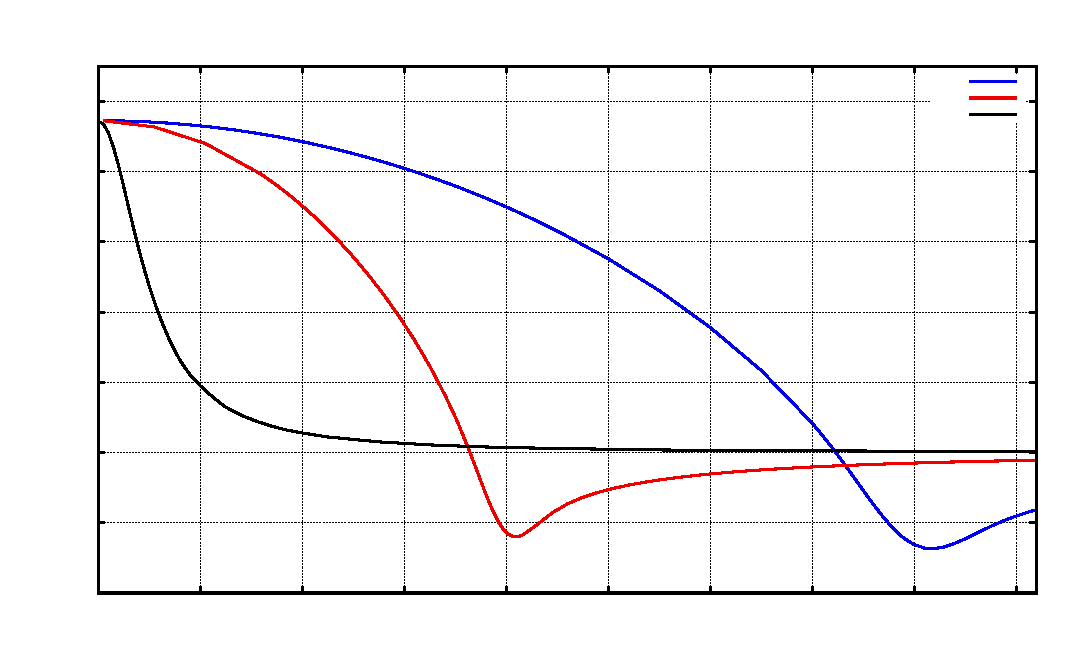
\includegraphics{m_over_m_xk_of_e_dc_B=diff}}%
    \gplfronttext
  \end{picture}%
\endgroup

	  \label{fig:effect1ive_mass_of_E_dc_different_B}
	  \caption{This plot corresponds to the one above (previous figure) and clearly shows how presence of magnetic field
	  pushes effective mass into negative region when slope of $v_{dr} = f(E_{dc})$ becomes negative.}
	\end{figure}
	\newpage
	\begin{figure}[H]
	  \centering
	  \normalsize % use normal font size in the figure
	  % GNUPLOT: LaTeX picture with Postscript
\begingroup
  \makeatletter
  \providecommand\color[2][]{%
    \GenericError{(gnuplot) \space\space\space\@spaces}{%
      Package color not loaded in conjunction with
      terminal option `colourtext'%
    }{See the gnuplot documentation for explanation.%
    }{Either use 'blacktext' in gnuplot or load the package
      color.sty in LaTeX.}%
    \renewcommand\color[2][]{}%
  }%
  \providecommand\includegraphics[2][]{%
    \GenericError{(gnuplot) \space\space\space\@spaces}{%
      Package graphicx or graphics not loaded%
    }{See the gnuplot documentation for explanation.%
    }{The gnuplot epslatex terminal needs graphicx.sty or graphics.sty.}%
    \renewcommand\includegraphics[2][]{}%
  }%
  \providecommand\rotatebox[2]{#2}%
  \@ifundefined{ifGPcolor}{%
    \newif\ifGPcolor
    \GPcolortrue
  }{}%
  \@ifundefined{ifGPblacktext}{%
    \newif\ifGPblacktext
    \GPblacktextfalse
  }{}%
  % define a \g@addto@macro without @ in the name:
  \let\gplgaddtomacro\g@addto@macro
  % define empty templates for all commands taking text:
  \gdef\gplbacktext{}%
  \gdef\gplfronttext{}%
  \makeatother
  \ifGPblacktext
    % no textcolor at all
    \def\colorrgb#1{}%
    \def\colorgray#1{}%
  \else
    % gray or color?
    \ifGPcolor
      \def\colorrgb#1{\color[rgb]{#1}}%
      \def\colorgray#1{\color[gray]{#1}}%
      \expandafter\def\csname LTw\endcsname{\color{white}}%
      \expandafter\def\csname LTb\endcsname{\color{black}}%
      \expandafter\def\csname LTa\endcsname{\color{black}}%
      \expandafter\def\csname LT0\endcsname{\color[rgb]{1,0,0}}%
      \expandafter\def\csname LT1\endcsname{\color[rgb]{0,1,0}}%
      \expandafter\def\csname LT2\endcsname{\color[rgb]{0,0,1}}%
      \expandafter\def\csname LT3\endcsname{\color[rgb]{1,0,1}}%
      \expandafter\def\csname LT4\endcsname{\color[rgb]{0,1,1}}%
      \expandafter\def\csname LT5\endcsname{\color[rgb]{1,1,0}}%
      \expandafter\def\csname LT6\endcsname{\color[rgb]{0,0,0}}%
      \expandafter\def\csname LT7\endcsname{\color[rgb]{1,0.3,0}}%
      \expandafter\def\csname LT8\endcsname{\color[rgb]{0.5,0.5,0.5}}%
    \else
      % gray
      \def\colorrgb#1{\color{black}}%
      \def\colorgray#1{\color[gray]{#1}}%
      \expandafter\def\csname LTw\endcsname{\color{white}}%
      \expandafter\def\csname LTb\endcsname{\color{black}}%
      \expandafter\def\csname LTa\endcsname{\color{black}}%
      \expandafter\def\csname LT0\endcsname{\color{black}}%
      \expandafter\def\csname LT1\endcsname{\color{black}}%
      \expandafter\def\csname LT2\endcsname{\color{black}}%
      \expandafter\def\csname LT3\endcsname{\color{black}}%
      \expandafter\def\csname LT4\endcsname{\color{black}}%
      \expandafter\def\csname LT5\endcsname{\color{black}}%
      \expandafter\def\csname LT6\endcsname{\color{black}}%
      \expandafter\def\csname LT7\endcsname{\color{black}}%
      \expandafter\def\csname LT8\endcsname{\color{black}}%
    \fi
  \fi
  \setlength{\unitlength}{0.0500bp}%
  \begin{picture}(10080.00,6048.00)%
    \gplgaddtomacro\gplbacktext{%
      \csname LTb\endcsname%
      \put(880,512){\makebox(0,0)[r]{\strut{}-0.015}}%
      \csname LTb\endcsname%
      \put(880,1152){\makebox(0,0)[r]{\strut{}-0.01}}%
      \csname LTb\endcsname%
      \put(880,1792){\makebox(0,0)[r]{\strut{}-0.005}}%
      \csname LTb\endcsname%
      \put(880,2432){\makebox(0,0)[r]{\strut{} 0}}%
      \csname LTb\endcsname%
      \put(880,3071){\makebox(0,0)[r]{\strut{} 0.005}}%
      \csname LTb\endcsname%
      \put(880,3711){\makebox(0,0)[r]{\strut{} 0.01}}%
      \csname LTb\endcsname%
      \put(880,4351){\makebox(0,0)[r]{\strut{} 0.015}}%
      \csname LTb\endcsname%
      \put(880,4991){\makebox(0,0)[r]{\strut{} 0.02}}%
      \csname LTb\endcsname%
      \put(976,352){\makebox(0,0){\strut{} 0}}%
      \csname LTb\endcsname%
      \put(2445,352){\makebox(0,0){\strut{} 2}}%
      \csname LTb\endcsname%
      \put(3914,352){\makebox(0,0){\strut{} 4}}%
      \csname LTb\endcsname%
      \put(5383,352){\makebox(0,0){\strut{} 6}}%
      \csname LTb\endcsname%
      \put(6852,352){\makebox(0,0){\strut{} 8}}%
      \csname LTb\endcsname%
      \put(8321,352){\makebox(0,0){\strut{} 10}}%
      \csname LTb\endcsname%
      \put(9790,352){\makebox(0,0){\strut{} 12}}%
      \put(128,3039){\rotatebox{-270}{\makebox(0,0){\strut{}$Absorption$}}}%
      \put(5383,112){\makebox(0,0){\strut{}$\omega$}}%
      \put(5383,5807){\makebox(0,0){\strut{}Absoprtion $A$ as a function of $\omega$. $\mu=116$, $\alpha=0.9496$, $E_{\omega}=0.1$, $E_{dc}=[0,6.4]$, $B=4$}}%
    }%
    \gplgaddtomacro\gplfronttext{%
      \csname LTb\endcsname%
      \put(9055,5424){\makebox(0,0)[r]{\strut{}$\mu=116, B=4$}}%
      \csname LTb\endcsname%
      \put(9055,5264){\makebox(0,0)[r]{\strut{}$\mu=116, B=0$ Bloch gain}}%
    }%
    \gplbacktext
    \put(0,0){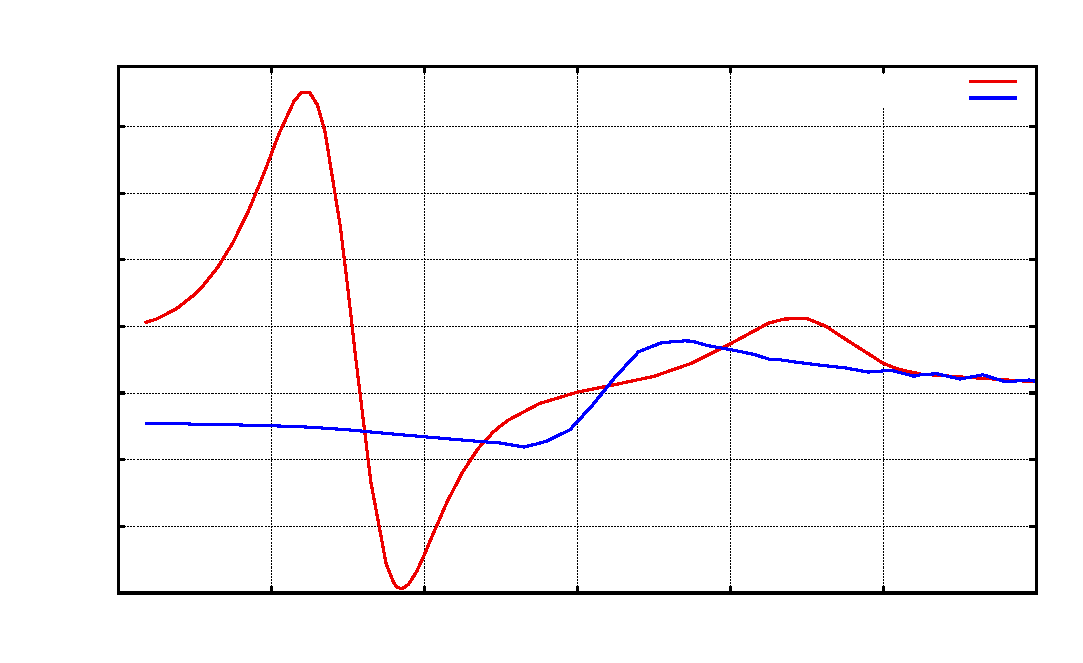
\includegraphics{cycl_vs_bloch_gain}}%
    \gplfronttext
  \end{picture}%
\endgroup

	  \label{fig:cycl_vs_bloch_gain}
	  \caption{In this picture we are drawing absorption as a function of $\tilde{\omega}$ with magnetic field turned on
	  $B = 4$ and turned off $B = 0$. We take $E_{dc} = 6.5$, which for $B = 4$ corresponds to plot (b) in figure 
	  \ref{fig:map_of_absorption_and_profiles_for_three_different_E_dc_B=4}. We can see that both, negative and 
	  positive absorption are much stronger than for corresponding Bloch regime ($B = 0$)}
	\end{figure}	
	\newpage
	\begin{figure}[H]
	  \centering
	  \normalsize % use normal font size in the figure
	  % GNUPLOT: LaTeX picture with Postscript
\begingroup
  \makeatletter
  \providecommand\color[2][]{%
    \GenericError{(gnuplot) \space\space\space\@spaces}{%
      Package color not loaded in conjunction with
      terminal option `colourtext'%
    }{See the gnuplot documentation for explanation.%
    }{Either use 'blacktext' in gnuplot or load the package
      color.sty in LaTeX.}%
    \renewcommand\color[2][]{}%
  }%
  \providecommand\includegraphics[2][]{%
    \GenericError{(gnuplot) \space\space\space\@spaces}{%
      Package graphicx or graphics not loaded%
    }{See the gnuplot documentation for explanation.%
    }{The gnuplot epslatex terminal needs graphicx.sty or graphics.sty.}%
    \renewcommand\includegraphics[2][]{}%
  }%
  \providecommand\rotatebox[2]{#2}%
  \@ifundefined{ifGPcolor}{%
    \newif\ifGPcolor
    \GPcolortrue
  }{}%
  \@ifundefined{ifGPblacktext}{%
    \newif\ifGPblacktext
    \GPblacktextfalse
  }{}%
  % define a \g@addto@macro without @ in the name:
  \let\gplgaddtomacro\g@addto@macro
  % define empty templates for all commands taking text:
  \gdef\gplbacktext{}%
  \gdef\gplfronttext{}%
  \makeatother
  \ifGPblacktext
    % no textcolor at all
    \def\colorrgb#1{}%
    \def\colorgray#1{}%
  \else
    % gray or color?
    \ifGPcolor
      \def\colorrgb#1{\color[rgb]{#1}}%
      \def\colorgray#1{\color[gray]{#1}}%
      \expandafter\def\csname LTw\endcsname{\color{white}}%
      \expandafter\def\csname LTb\endcsname{\color{black}}%
      \expandafter\def\csname LTa\endcsname{\color{black}}%
      \expandafter\def\csname LT0\endcsname{\color[rgb]{1,0,0}}%
      \expandafter\def\csname LT1\endcsname{\color[rgb]{0,1,0}}%
      \expandafter\def\csname LT2\endcsname{\color[rgb]{0,0,1}}%
      \expandafter\def\csname LT3\endcsname{\color[rgb]{1,0,1}}%
      \expandafter\def\csname LT4\endcsname{\color[rgb]{0,1,1}}%
      \expandafter\def\csname LT5\endcsname{\color[rgb]{1,1,0}}%
      \expandafter\def\csname LT6\endcsname{\color[rgb]{0,0,0}}%
      \expandafter\def\csname LT7\endcsname{\color[rgb]{1,0.3,0}}%
      \expandafter\def\csname LT8\endcsname{\color[rgb]{0.5,0.5,0.5}}%
    \else
      % gray
      \def\colorrgb#1{\color{black}}%
      \def\colorgray#1{\color[gray]{#1}}%
      \expandafter\def\csname LTw\endcsname{\color{white}}%
      \expandafter\def\csname LTb\endcsname{\color{black}}%
      \expandafter\def\csname LTa\endcsname{\color{black}}%
      \expandafter\def\csname LT0\endcsname{\color{black}}%
      \expandafter\def\csname LT1\endcsname{\color{black}}%
      \expandafter\def\csname LT2\endcsname{\color{black}}%
      \expandafter\def\csname LT3\endcsname{\color{black}}%
      \expandafter\def\csname LT4\endcsname{\color{black}}%
      \expandafter\def\csname LT5\endcsname{\color{black}}%
      \expandafter\def\csname LT6\endcsname{\color{black}}%
      \expandafter\def\csname LT7\endcsname{\color{black}}%
      \expandafter\def\csname LT8\endcsname{\color{black}}%
    \fi
  \fi
  \setlength{\unitlength}{0.0500bp}%
  \begin{picture}(10080.00,6048.00)%
    \gplgaddtomacro\gplbacktext{%
      \csname LTb\endcsname%
      \put(784,512){\makebox(0,0)[r]{\strut{} 0}}%
      \csname LTb\endcsname%
      \put(784,1466){\makebox(0,0)[r]{\strut{} 0.01}}%
      \csname LTb\endcsname%
      \put(784,2420){\makebox(0,0)[r]{\strut{} 0.02}}%
      \csname LTb\endcsname%
      \put(784,3373){\makebox(0,0)[r]{\strut{} 0.03}}%
      \csname LTb\endcsname%
      \put(784,4327){\makebox(0,0)[r]{\strut{} 0.04}}%
      \csname LTb\endcsname%
      \put(784,5281){\makebox(0,0)[r]{\strut{} 0.05}}%
      \csname LTb\endcsname%
      \put(880,352){\makebox(0,0){\strut{} 0}}%
      \csname LTb\endcsname%
      \put(2365,352){\makebox(0,0){\strut{} 2}}%
      \csname LTb\endcsname%
      \put(3850,352){\makebox(0,0){\strut{} 4}}%
      \csname LTb\endcsname%
      \put(5335,352){\makebox(0,0){\strut{} 6}}%
      \csname LTb\endcsname%
      \put(6820,352){\makebox(0,0){\strut{} 8}}%
      \csname LTb\endcsname%
      \put(8305,352){\makebox(0,0){\strut{} 10}}%
      \csname LTb\endcsname%
      \put(9790,352){\makebox(0,0){\strut{} 12}}%
      \put(128,3039){\rotatebox{-270}{\makebox(0,0){\strut{}$Absorption$}}}%
      \put(5335,112){\makebox(0,0){\strut{}$\omega$}}%
      \put(5335,5807){\makebox(0,0){\strut{}Absoprtion $A$ as a function of $\omega$. $\mu=116$, $\alpha=0.9496$, $B=4$, $E_{\omega}=0.1$, $E_{dc}=0$}}%
    }%
    \gplgaddtomacro\gplfronttext{%
      \csname LTb\endcsname%
      \put(9055,5424){\makebox(0,0)[r]{\strut{}$\mu=116$}}%
      \csname LTb\endcsname%
      \put(9055,5264){\makebox(0,0)[r]{\strut{}$\mu=\infty$}}%
    }%
    \gplbacktext
    \put(0,0){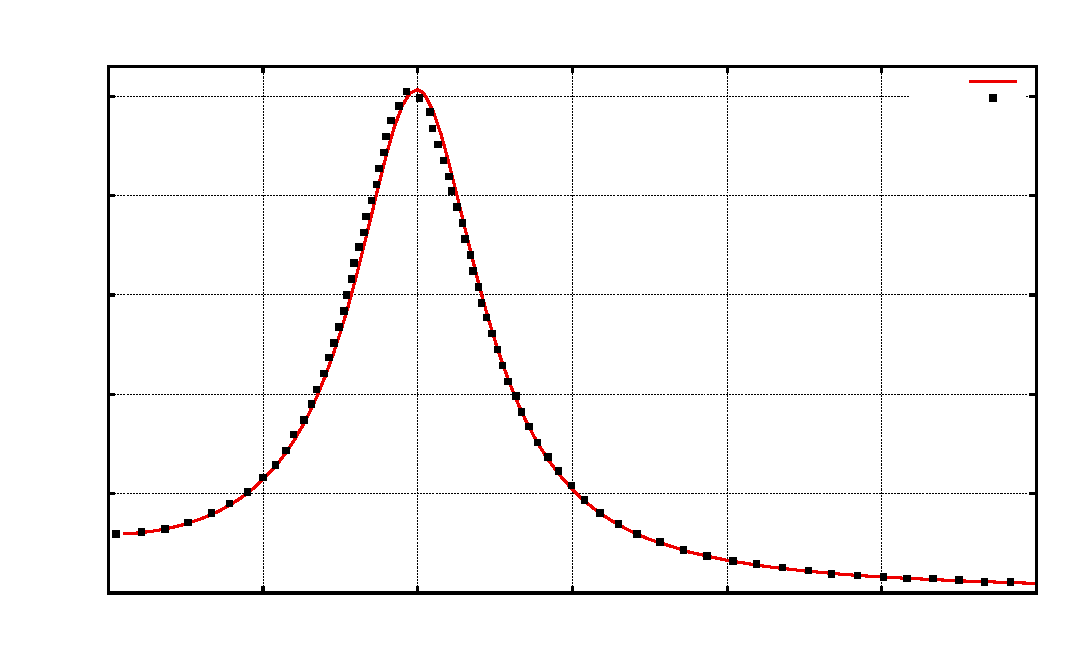
\includegraphics{lorentz_gain}}%
    \gplfronttext
  \end{picture}%
\endgroup

	  \label{fig:lorentz_gain}
	  \caption{In this picture we validate our algorithm and code by comparing absorption at finite, but very low 
	  temperature $\mu = 113$, with well known Lorentz gain profile shown in black squares, which corresponds 
	  to $\mu = \infty$. Plot of black squares was scanned from \cite{PhysRevLett.103.117401} (Figure 1c). 
	  You can see here good correspondence proving correctness of of our approach.}
	\end{figure}	
	\begin{figure}[H]
	  \centering
	  \normalsize % use normal font size in the figure
	  % GNUPLOT: LaTeX picture with Postscript
\begingroup
  \makeatletter
  \providecommand\color[2][]{%
    \GenericError{(gnuplot) \space\space\space\@spaces}{%
      Package color not loaded in conjunction with
      terminal option `colourtext'%
    }{See the gnuplot documentation for explanation.%
    }{Either use 'blacktext' in gnuplot or load the package
      color.sty in LaTeX.}%
    \renewcommand\color[2][]{}%
  }%
  \providecommand\includegraphics[2][]{%
    \GenericError{(gnuplot) \space\space\space\@spaces}{%
      Package graphicx or graphics not loaded%
    }{See the gnuplot documentation for explanation.%
    }{The gnuplot epslatex terminal needs graphicx.sty or graphics.sty.}%
    \renewcommand\includegraphics[2][]{}%
  }%
  \providecommand\rotatebox[2]{#2}%
  \@ifundefined{ifGPcolor}{%
    \newif\ifGPcolor
    \GPcolortrue
  }{}%
  \@ifundefined{ifGPblacktext}{%
    \newif\ifGPblacktext
    \GPblacktextfalse
  }{}%
  % define a \g@addto@macro without @ in the name:
  \let\gplgaddtomacro\g@addto@macro
  % define empty templates for all commands taking text:
  \gdef\gplbacktext{}%
  \gdef\gplfronttext{}%
  \makeatother
  \ifGPblacktext
    % no textcolor at all
    \def\colorrgb#1{}%
    \def\colorgray#1{}%
  \else
    % gray or color?
    \ifGPcolor
      \def\colorrgb#1{\color[rgb]{#1}}%
      \def\colorgray#1{\color[gray]{#1}}%
      \expandafter\def\csname LTw\endcsname{\color{white}}%
      \expandafter\def\csname LTb\endcsname{\color{black}}%
      \expandafter\def\csname LTa\endcsname{\color{black}}%
      \expandafter\def\csname LT0\endcsname{\color[rgb]{1,0,0}}%
      \expandafter\def\csname LT1\endcsname{\color[rgb]{0,1,0}}%
      \expandafter\def\csname LT2\endcsname{\color[rgb]{0,0,1}}%
      \expandafter\def\csname LT3\endcsname{\color[rgb]{1,0,1}}%
      \expandafter\def\csname LT4\endcsname{\color[rgb]{0,1,1}}%
      \expandafter\def\csname LT5\endcsname{\color[rgb]{1,1,0}}%
      \expandafter\def\csname LT6\endcsname{\color[rgb]{0,0,0}}%
      \expandafter\def\csname LT7\endcsname{\color[rgb]{1,0.3,0}}%
      \expandafter\def\csname LT8\endcsname{\color[rgb]{0.5,0.5,0.5}}%
    \else
      % gray
      \def\colorrgb#1{\color{black}}%
      \def\colorgray#1{\color[gray]{#1}}%
      \expandafter\def\csname LTw\endcsname{\color{white}}%
      \expandafter\def\csname LTb\endcsname{\color{black}}%
      \expandafter\def\csname LTa\endcsname{\color{black}}%
      \expandafter\def\csname LT0\endcsname{\color{black}}%
      \expandafter\def\csname LT1\endcsname{\color{black}}%
      \expandafter\def\csname LT2\endcsname{\color{black}}%
      \expandafter\def\csname LT3\endcsname{\color{black}}%
      \expandafter\def\csname LT4\endcsname{\color{black}}%
      \expandafter\def\csname LT5\endcsname{\color{black}}%
      \expandafter\def\csname LT6\endcsname{\color{black}}%
      \expandafter\def\csname LT7\endcsname{\color{black}}%
      \expandafter\def\csname LT8\endcsname{\color{black}}%
    \fi
  \fi
  \setlength{\unitlength}{0.0500bp}%
  \begin{picture}(10080.00,6048.00)%
    \gplgaddtomacro\gplbacktext{%
      \csname LTb\endcsname%
      \put(880,512){\makebox(0,0)[r]{\strut{}-0.01}}%
      \csname LTb\endcsname%
      \put(880,1144){\makebox(0,0)[r]{\strut{}-0.005}}%
      \csname LTb\endcsname%
      \put(880,1776){\makebox(0,0)[r]{\strut{} 0}}%
      \csname LTb\endcsname%
      \put(880,2408){\makebox(0,0)[r]{\strut{} 0.005}}%
      \csname LTb\endcsname%
      \put(880,3040){\makebox(0,0)[r]{\strut{} 0.01}}%
      \csname LTb\endcsname%
      \put(880,3671){\makebox(0,0)[r]{\strut{} 0.015}}%
      \csname LTb\endcsname%
      \put(880,4303){\makebox(0,0)[r]{\strut{} 0.02}}%
      \csname LTb\endcsname%
      \put(880,4935){\makebox(0,0)[r]{\strut{} 0.025}}%
      \csname LTb\endcsname%
      \put(880,5567){\makebox(0,0)[r]{\strut{} 0.03}}%
      \csname LTb\endcsname%
      \put(976,352){\makebox(0,0){\strut{} 0}}%
      \csname LTb\endcsname%
      \put(2445,352){\makebox(0,0){\strut{} 2}}%
      \csname LTb\endcsname%
      \put(3914,352){\makebox(0,0){\strut{} 4}}%
      \csname LTb\endcsname%
      \put(5383,352){\makebox(0,0){\strut{} 6}}%
      \csname LTb\endcsname%
      \put(6852,352){\makebox(0,0){\strut{} 8}}%
      \csname LTb\endcsname%
      \put(8321,352){\makebox(0,0){\strut{} 10}}%
      \csname LTb\endcsname%
      \put(9790,352){\makebox(0,0){\strut{} 12}}%
      \put(128,3039){\rotatebox{-270}{\makebox(0,0){\strut{}$Absorption$}}}%
      \put(5383,112){\makebox(0,0){\strut{}$\omega$}}%
      \put(5383,5807){\makebox(0,0){\strut{}Absoprtion $A$ as a function of $\omega$. $\mu=116$, $\alpha=0.9496$, $B=4$, $E_{\omega}=0.1$, $E_{dc}=6$}}%
    }%
    \gplgaddtomacro\gplfronttext{%
      \csname LTb\endcsname%
      \put(9055,5424){\makebox(0,0)[r]{\strut{}$\mu=116$}}%
      \csname LTb\endcsname%
      \put(9055,5264){\makebox(0,0)[r]{\strut{}$\mu=\infty$}}%
    }%
    \gplbacktext
    \put(0,0){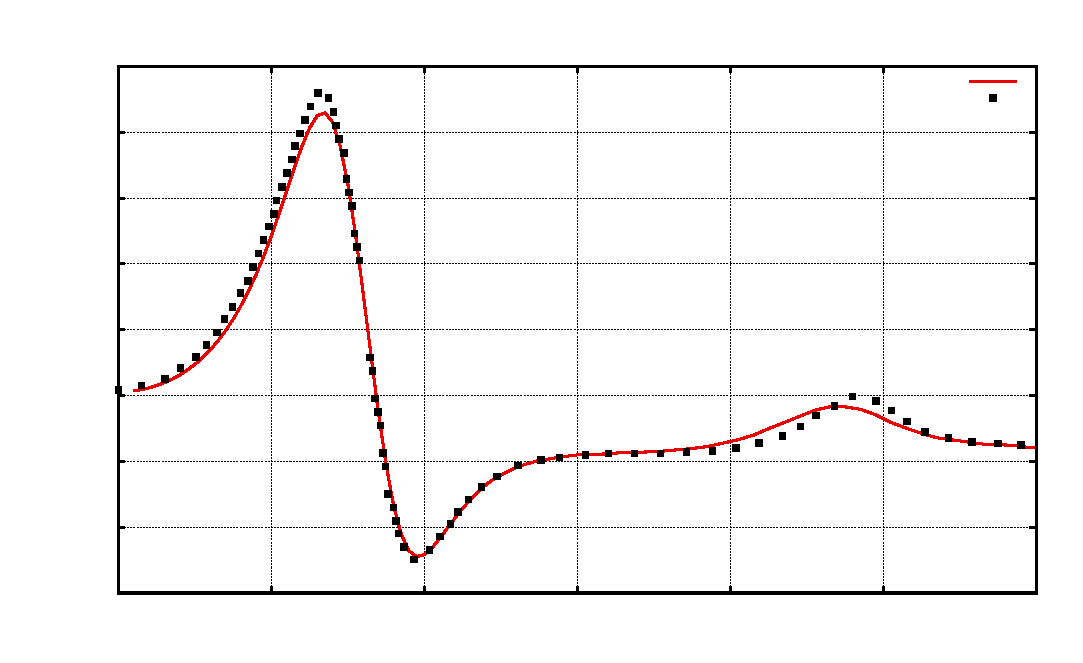
\includegraphics{gain_at_E_dc=6}}%
    \gplfronttext
  \end{picture}%
\endgroup

	  \label{fig:gain_at_E_dc=6}
	  \caption{Similarly to previous plot, in this figure we validate numerical code by comparing solution 
	  at $\mu = \infty$, shown in the black squares, from \cite{PhysRevLett.103.117401} (Figure 1d) with 
	  numerical solution (in red) $\mu = 116$, which is close enough to 0 temperature. You can see here good
	  correspondence proving correctness of of our approach.}
	\end{figure}
\end{document}
  
